\documentclass[12pt]{article}

%   Packages  
\usepackage[utf8]{inputenc}
\usepackage[margin=1in]{geometry}
\usepackage{amsmath, amssymb, amsfonts}
\usepackage{graphicx}
\usepackage{grffile}  % handle paths with spaces (e.g. "ACV Assignment 2")
\usepackage{hyperref}
\usepackage{enumerate}
\usepackage{mathpazo}
\usepackage{float}
\usepackage{subcaption} % Added for subfigures
\usepackage{listings}
\usepackage{xcolor}

\definecolor{codegreen}{rgb}{0,0.6,0}
\definecolor{codegray}{rgb}{0.5,0.5,0.5}
\definecolor{codepurple}{rgb}{0.58,0,0.82}
\definecolor{backcolour}{rgb}{0.95,0.95,0.92}

\lstdefinestyle{mystyle}{
    backgroundcolor=\color{backcolour},   
    commentstyle=\color{codegreen},
    keywordstyle=\color{magenta},
    numberstyle=\tiny\color{codegray},
    stringstyle=\color{codepurple},
    basicstyle=\ttfamily\footnotesize,
    breakatwhitespace=false,         
    breaklines=true,                 
    captionpos=b,                    
    keepspaces=true,                 
    numbers=left,                    
    numbersep=5pt,                  
    showspaces=false,                
    showstringspaces=false,
    showtabs=false,                  
    tabsize=2
}

\lstset{style=mystyle}

% --- Document Information ---
\title{18-799 Applied Computer Vision \\ Homework 2}
\author{\textbf{Name:} Edward Ajayi \\ \textbf{Andrew ID:} eaajayi \\ \textbf{Semester:} Spring 2026}
\date{\textbf{Date:} \today}

% Graphics path: compile from the folder containing hw2.tex; keep Q3/Q4 images in Assets/
\graphicspath{{./Assets/}}

\begin{document}

\maketitle
\newpage

% \section*{Introduction}
% In this assignment, we explore key computer vision techniques, including object counting, line detection, image compression, and data augmentation. We apply these techniques to practical problems such as inventory management and chess board alignment using the OpenCV library\cite{opencv_docs}.

\section{Counting Objects}

\subsection{Implementation of Naive Algorithm}
This has been implemented in the notebook file.

\subsection{Methodology}
To count objects in an image, we implemented a naive pipeline consisting of the following steps:
\begin{enumerate}
    \item \textbf{Grayscale Conversion:} Converted the image to grayscale ($Y = 0.299R + 0.587G + 0.114B$) to simplify processing.
    \item \textbf{Gaussian Blur:} Applied a Gaussian kernel to reduce high-frequency noise that could be mistaken for edges.
    \item \textbf{Canny Edge Detection:} Detected edges using the Canny algorithm\cite{canny1986computational} (gradient calculation, non-maximum suppression, hysteresis thresholding).
    \item \textbf{Contour Finding:} Retrieved external contours from the binary edge map.
    \item \textbf{Counting:} The number of contours corresponds to the number of objects.
\end{enumerate}

\begin{figure}[H]
    \centering
    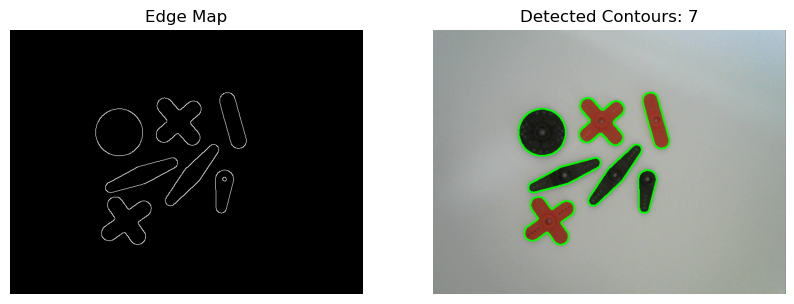
\includegraphics[width=\textwidth]{q1_results.png}
    \caption{Object counting results: (Left) Canny Edge Map, (Right) Detected Contours showing 7 distinct objects.}
    \label{fig:q1_results}
\end{figure}

\subsection{Experimentation \& Parameter Tuning}
For touching objects (as seen in the provided dataset), the naive method fails because boundaries merge. We experimented with \textbf{Morphological Operations} and the \textbf{Watershed Algorithm}\cite{beucher1979watersheds}. The critical parameter was the distance transform threshold factor $\alpha$.

\begin{table}[H]
\centering
\begin{tabular}{|c|c|c|l|}
\hline
\textbf{$\alpha$ (Threshold)} & \textbf{Opening Iterations} & \textbf{Count} & \textbf{Outcome/Analysis} \\ \hline
0.5 & 2 & 2 & Threshold too high; only thickest objects survived. \\ \hline
0.1 & 2 & 10 & Threshold too low; thin objects merged. \\ \hline
\textbf{0.15} & \textbf{1} & \textbf{13} & \textbf{Optimal.} All objects separated correctly. \\ \hline
\end{tabular}
\caption{Parameter tuning results for separating touching objects.}
\label{tab:q1_tuning}
\end{table}

\begin{figure}[H]
    \centering
    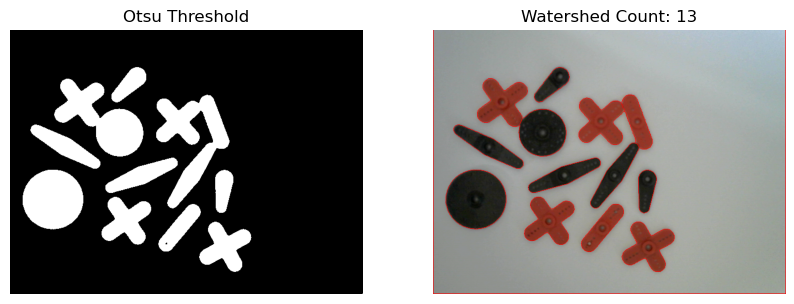
\includegraphics[width=\textwidth]{q1_watershed.png}
    \caption{Separation of touching objects using the Watershed algorithm with optimized parameters ($\alpha=0.15$, 1 iteration). The algorithm correctly identified 13 objects.}
    \label{fig:q1_watershed}
\end{figure}

\subsection{Real World Experimentation}
We performed two real-world experiments to test the robustness of our counting algorithm.

\begin{figure}[H]
    \centering
    \begin{subfigure}[b]{0.48\textwidth}
        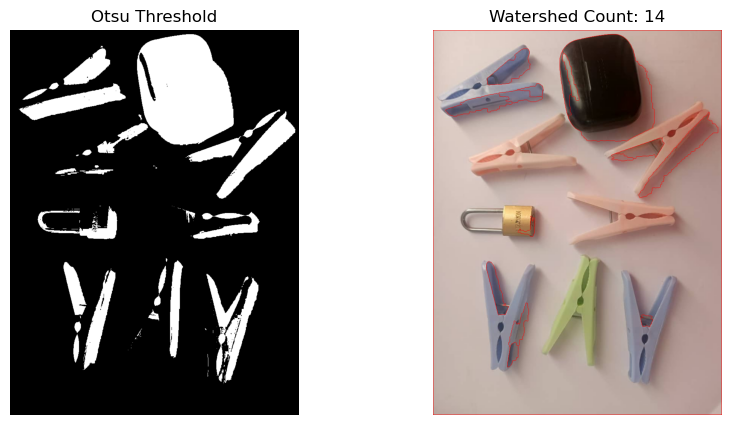
\includegraphics[width=\textwidth]{q1_realworld_clips.png}
        \caption{Experiment 1: Clothes Clips (Inflated Count)}
        \label{fig:q1_clips}
    \end{subfigure}
    \hfill
    \begin{subfigure}[b]{0.48\textwidth}
        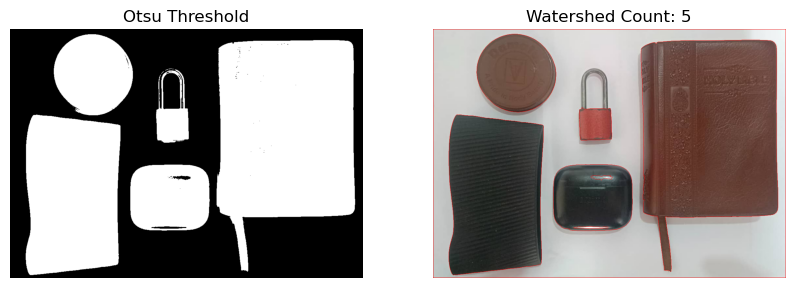
\includegraphics[width=\textwidth]{q1_realworld_objects.png}
        \caption{Experiment 2: Diverse Objects (Correct Count)}
        \label{fig:q1_objects}
    \end{subfigure}
    \caption{Real-world results. (a) Clothes clips are over-counted due to internal separable lines. (b) Diverse objects (wallet, lock, etc.) are correctly segmented.}
    \label{fig:q1_realworld}
\end{figure}

\begin{itemize}
    \item \textbf{Experiment 1 (Clips):} We tested the algorithm on clothes clips (Figure \ref{fig:q1_clips}). The result showed an inflated count. This is likely because the clips have a discernible separable line in the middle (the metal spring mechanism), which the edge detector interprets as a boundary, causing the algorithm to split a single object into two.
    \item \textbf{Experiment 2 (Diverse Objects):} We tested on a set of distinct objects including a wallet, lock, and case (Figure \ref{fig:q1_objects}). Here, the algorithm performed correctly. Unlike the clips, these objects have solid, uniform shapes without strong internal edges, allowing the Watershed algorithm to segment them accurately.
\end{itemize}

\subsection{Difficulties Faced \& Improvements}
The naive counting algorithm faced several challenges in the real-world scenario:
\begin{enumerate}
    \item \textbf{Touching Objects:} The naive method treats touching objects as a single contour. \textit{Improvement:} Use Watershed algorithm or morphological erosion to separate them.
    \item \textbf{Shadows:} Strong lighting created shadows interpreted as extra edges. \textit{Improvement:} Use diffuse lighting or background subtraction algorithms.
    \item \textbf{Reflections:} Shiny plastic parts created ``holes'' in the edge map. \textit{Improvement:} Use polarizing filters or hole-filling morphological operations (Closing).
\end{enumerate}

\subsection{Other Real World Scenarios}
Counting objects is useful in various domains:
\begin{itemize}
    \item \textbf{Traffic Monitoring:} Counting vehicles on a highway for congestion analysis.
    \item \textbf{Microbiology:} Counting bacteria colonies or blood cells on a slide.
    \item \textbf{Manufacturing:} Counting products on a conveyor belt for quality control and yield estimation.
    \item \textbf{Crowd Control:} Estimating the number of people in a specific zone for safety.
\end{itemize}

\subsection{Bonus: Evaluating Image-Based Object Counting on Video}
We applied the naive object counting pipeline to a video sequence (\texttt{Assets/bonus\_output.mp4}) containing 3--5 objects.
\begin{itemize}
    \item \textbf{Observations:} The count fluctuates significantly as objects move or lighting changes. The count is rarely stable.
    \item \textbf{Limitations Identified:}
    \begin{enumerate}
        \item \textbf{Temporal Instability:} The algorithm processes each frame independently. Noise in one frame can cause a contour to split or disappear, leading to flickering counts.
        \item \textbf{Motion Blur:} Fast-moving objects blur, reducing edge strength. The Canny detector fails to find continuous edges, causing the object to be missed.
        \item \textbf{Occlusion:} When one object passes behind another, they merge into a single contour (count decreases by 1). The naive method offers no tracking or ID persistence.
    \end{enumerate}
\end{itemize}

\newpage
\section{Finding lines on a chessboard}

\subsection{Goal}
The objective is to automatically straighten a tilted image of a chessboard. This is a common preprocessing step in computer vision pipelines (e.g., OCR, document scanning) to standardize the input before further analysis.

\subsection{Methodology}
We implemented a geometric computer vision pipeline consisting of the following stages:

\begin{enumerate}
    \item \textbf{Preprocessing (Grayscale \& Blur):}
    We convert the image to grayscale as color is irrelevant for structural line detection. We then apply Gaussian Blur to suppress noise. Our experiments showed that a kernel size of $(5,5)$ was optimal for preserving grid lines while removing fine texture (like table grain). Larger kernels (e.g., $9 \times 9$) were too aggressive and blurred the grid lines themselves.
    
    \item \textbf{Contrast Enhancement (CLAHE):}
    Lighting on chessboards is often uneven due to reflections. We used Contrast Limited Adaptive Histogram Equalization (CLAHE)~\cite{zuiderveld1994clahe} with a clip limit of 2.0 and tile size $(8,8)$ to locally enhance contrast, ensuring grid lines are visible across the entire board.

    \item \textbf{Edge Detection (Canny):}
    We used the Canny edge detector~\cite{canny1986computational} with thresholds \textbf{100} and \textbf{200}. These higher thresholds (compared to the standard 50/150) helped filter out weaker edges from the background texture while keeping the strong board lines.

    \item \textbf{Line Detection (Hough Transform):}
    We used the Hough Transform~\cite{duda1972use} to detect lines. A line is represented in Hessian Normal form:
    \begin{equation}
        \rho = x \cos \theta + y \sin \theta
    \end{equation}
    The accumulator threshold was a critical parameter. A value of \textbf{300} was found to be the sweet spot. Lower values (200) resulted in hundreds of spurious lines from the wooden table grain, while higher values (500) missed legitimate grid lines.

    \item \textbf{Angle Analysis:}
    We analyzed the angles ($\theta$) of all detected lines to find the dominant orientation. The valid rotation angle was calculated by finding the difference between the dominant angle and the nearest rectilinear axis ($0^\circ, 90^\circ, 180^\circ$).

    \item \textbf{Image Rotation:}
    Using the calculated rotation angle $\phi$, we constructed a rotation matrix $M$:
    \begin{equation}
        M = \begin{bmatrix}
        \alpha & \beta & (1-\alpha)c_x - \beta c_y \\
        -\beta & \alpha & \beta c_x + (1-\alpha)c_y
        \end{bmatrix}
    \end{equation}
    where $\alpha = \cos \phi$ and $\beta = \sin \phi$. We used bilinear interpolation and edge replication to warp the image.
\end{enumerate}

\subsection{Experimentation \& Parameter Tuning}
We conducted extensive experiments to tune the Gaussian Blur kernel and Hough Transform threshold.

\subsubsection{Hough Transform Threshold}
The threshold determines the minimum number of votes to accept a line.
\begin{table}[H]
\centering
\begin{tabular}{|c|l|l|}
\hline
\textbf{Threshold} & \textbf{Result} & \textbf{Assessment} \\ \hline
200 & Hundreds of spurious lines (noise). & \textbf{Too Low} \\ \hline
\textbf{300} & \textbf{Clean detection of grid lines.} & \textbf{Optimal} \\ \hline
400--500 & Missed legitimate grid lines. & Too High \\ \hline
\end{tabular}
\caption{Effect of Hough Transform threshold on line detection quality.}
\label{tab:q2_threshold}
\end{table}

\subsubsection{Gaussian Blur Kernel}
The kernel size affects detail preservation.
\begin{table}[H]
\centering
\begin{tabular}{|c|l|}
\hline
\textbf{Kernel Size} & \textbf{Effect} \\ \hline
\textbf{(5, 5)} & \textbf{Optimal.} Preserves lines, removes noise. \\ \hline
(7, 7) & Missed middle lines; inconsistent. \\ \hline
(9, 9) & Too aggressive; blurred out grid lines. \\ \hline
\end{tabular}
\caption{Effect of Gaussian Blur kernel size.}
\label{tab:q2_blur}
\end{table}

\subsection{Results}
We applied the pipeline to all three provided chessboard images and one real-world object. Table~\ref{tab:q2_results} summarizes the detected dominant angles and the rotation corrections applied.

\begin{table}[H]
\centering
\begin{tabular}{|c|c|c|}
\hline
\textbf{Image} & \textbf{Dominant Angle} & \textbf{Rotation Applied} \\ \hline
\texttt{2a.jpg} & $90.00^\circ$ & $-0.00^\circ$ (already straight) \\ \hline
\texttt{2b.jpg} & $34.00^\circ$ & $-34.00^\circ$ \\ \hline
\texttt{2c.jpg} & $20.00^\circ$ & $-20.00^\circ$ \\ \hline
\texttt{cube} (Rubik's Cube) & $141.00^\circ$ & $39.00^\circ$ \\ \hline
\end{tabular}
\caption{Detected dominant angles and rotation corrections for each test image.}
\label{tab:q2_results}
\end{table}

\begin{figure}[H]
    \centering
    \begin{subfigure}[b]{0.32\textwidth}
        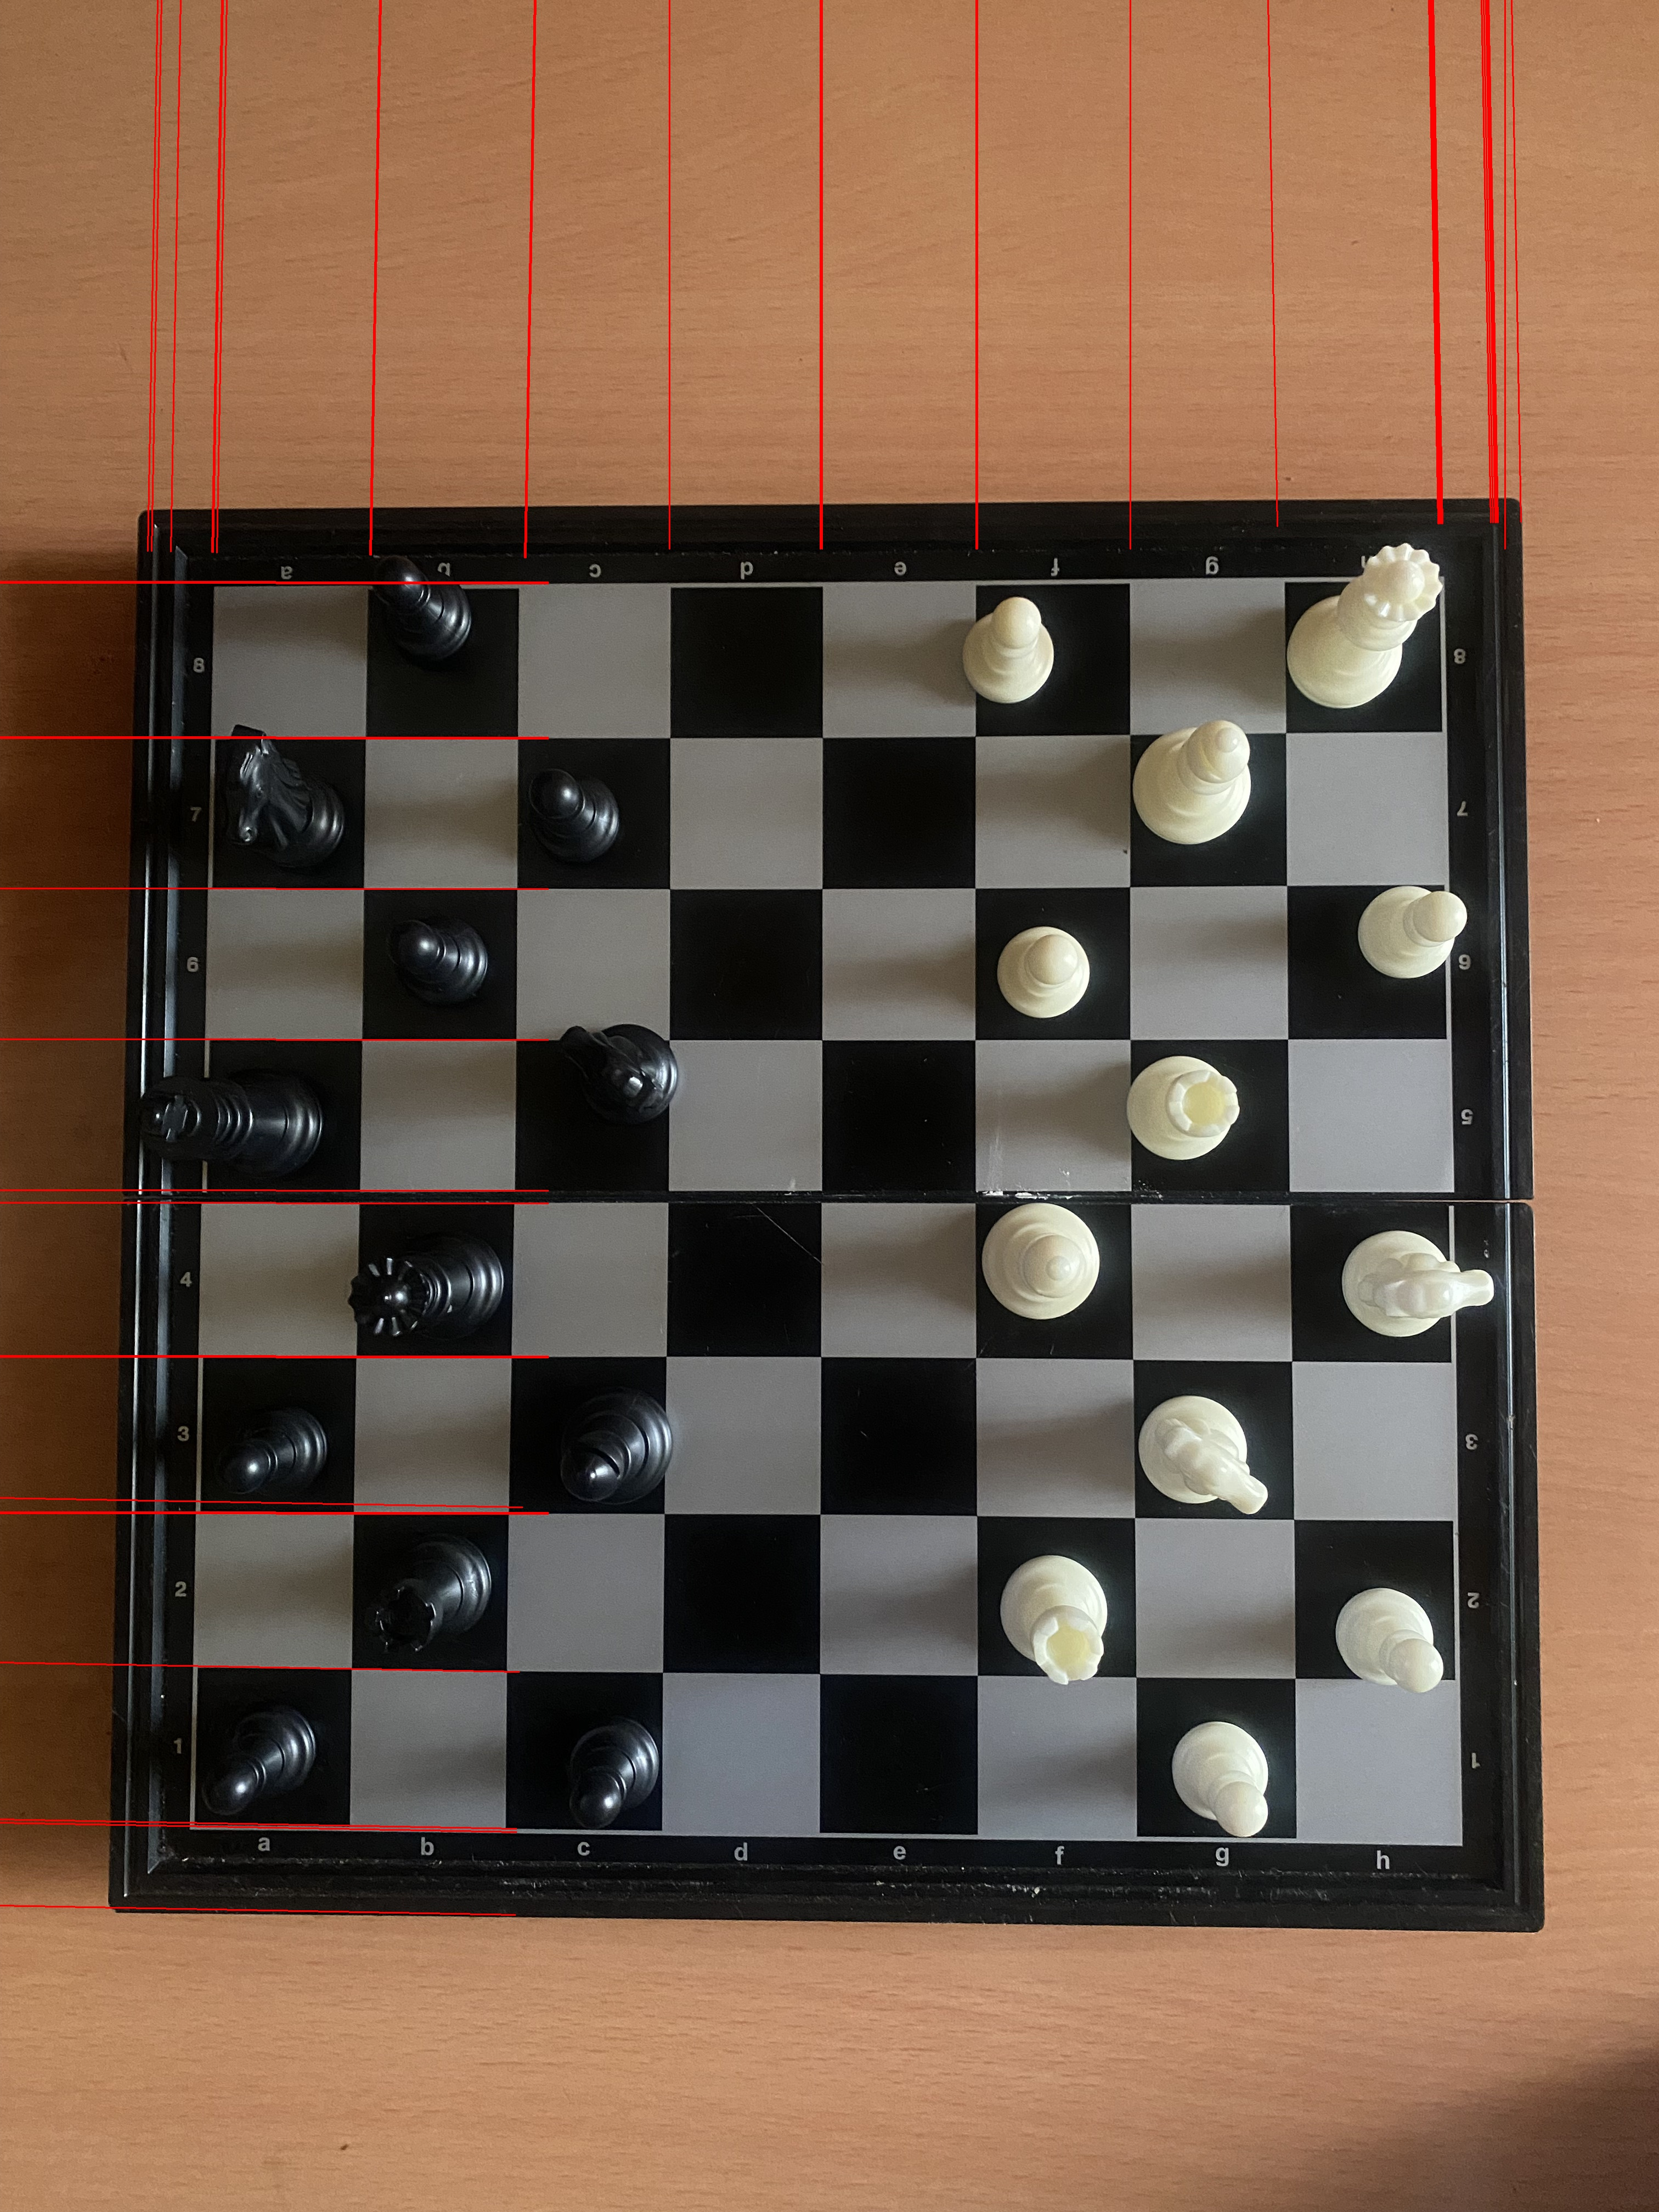
\includegraphics[width=\textwidth]{linesDetected2a.jpg}
        \caption{\texttt{2a} ($90^\circ$)}
    \end{subfigure}
    \hfill
    \begin{subfigure}[b]{0.32\textwidth}
        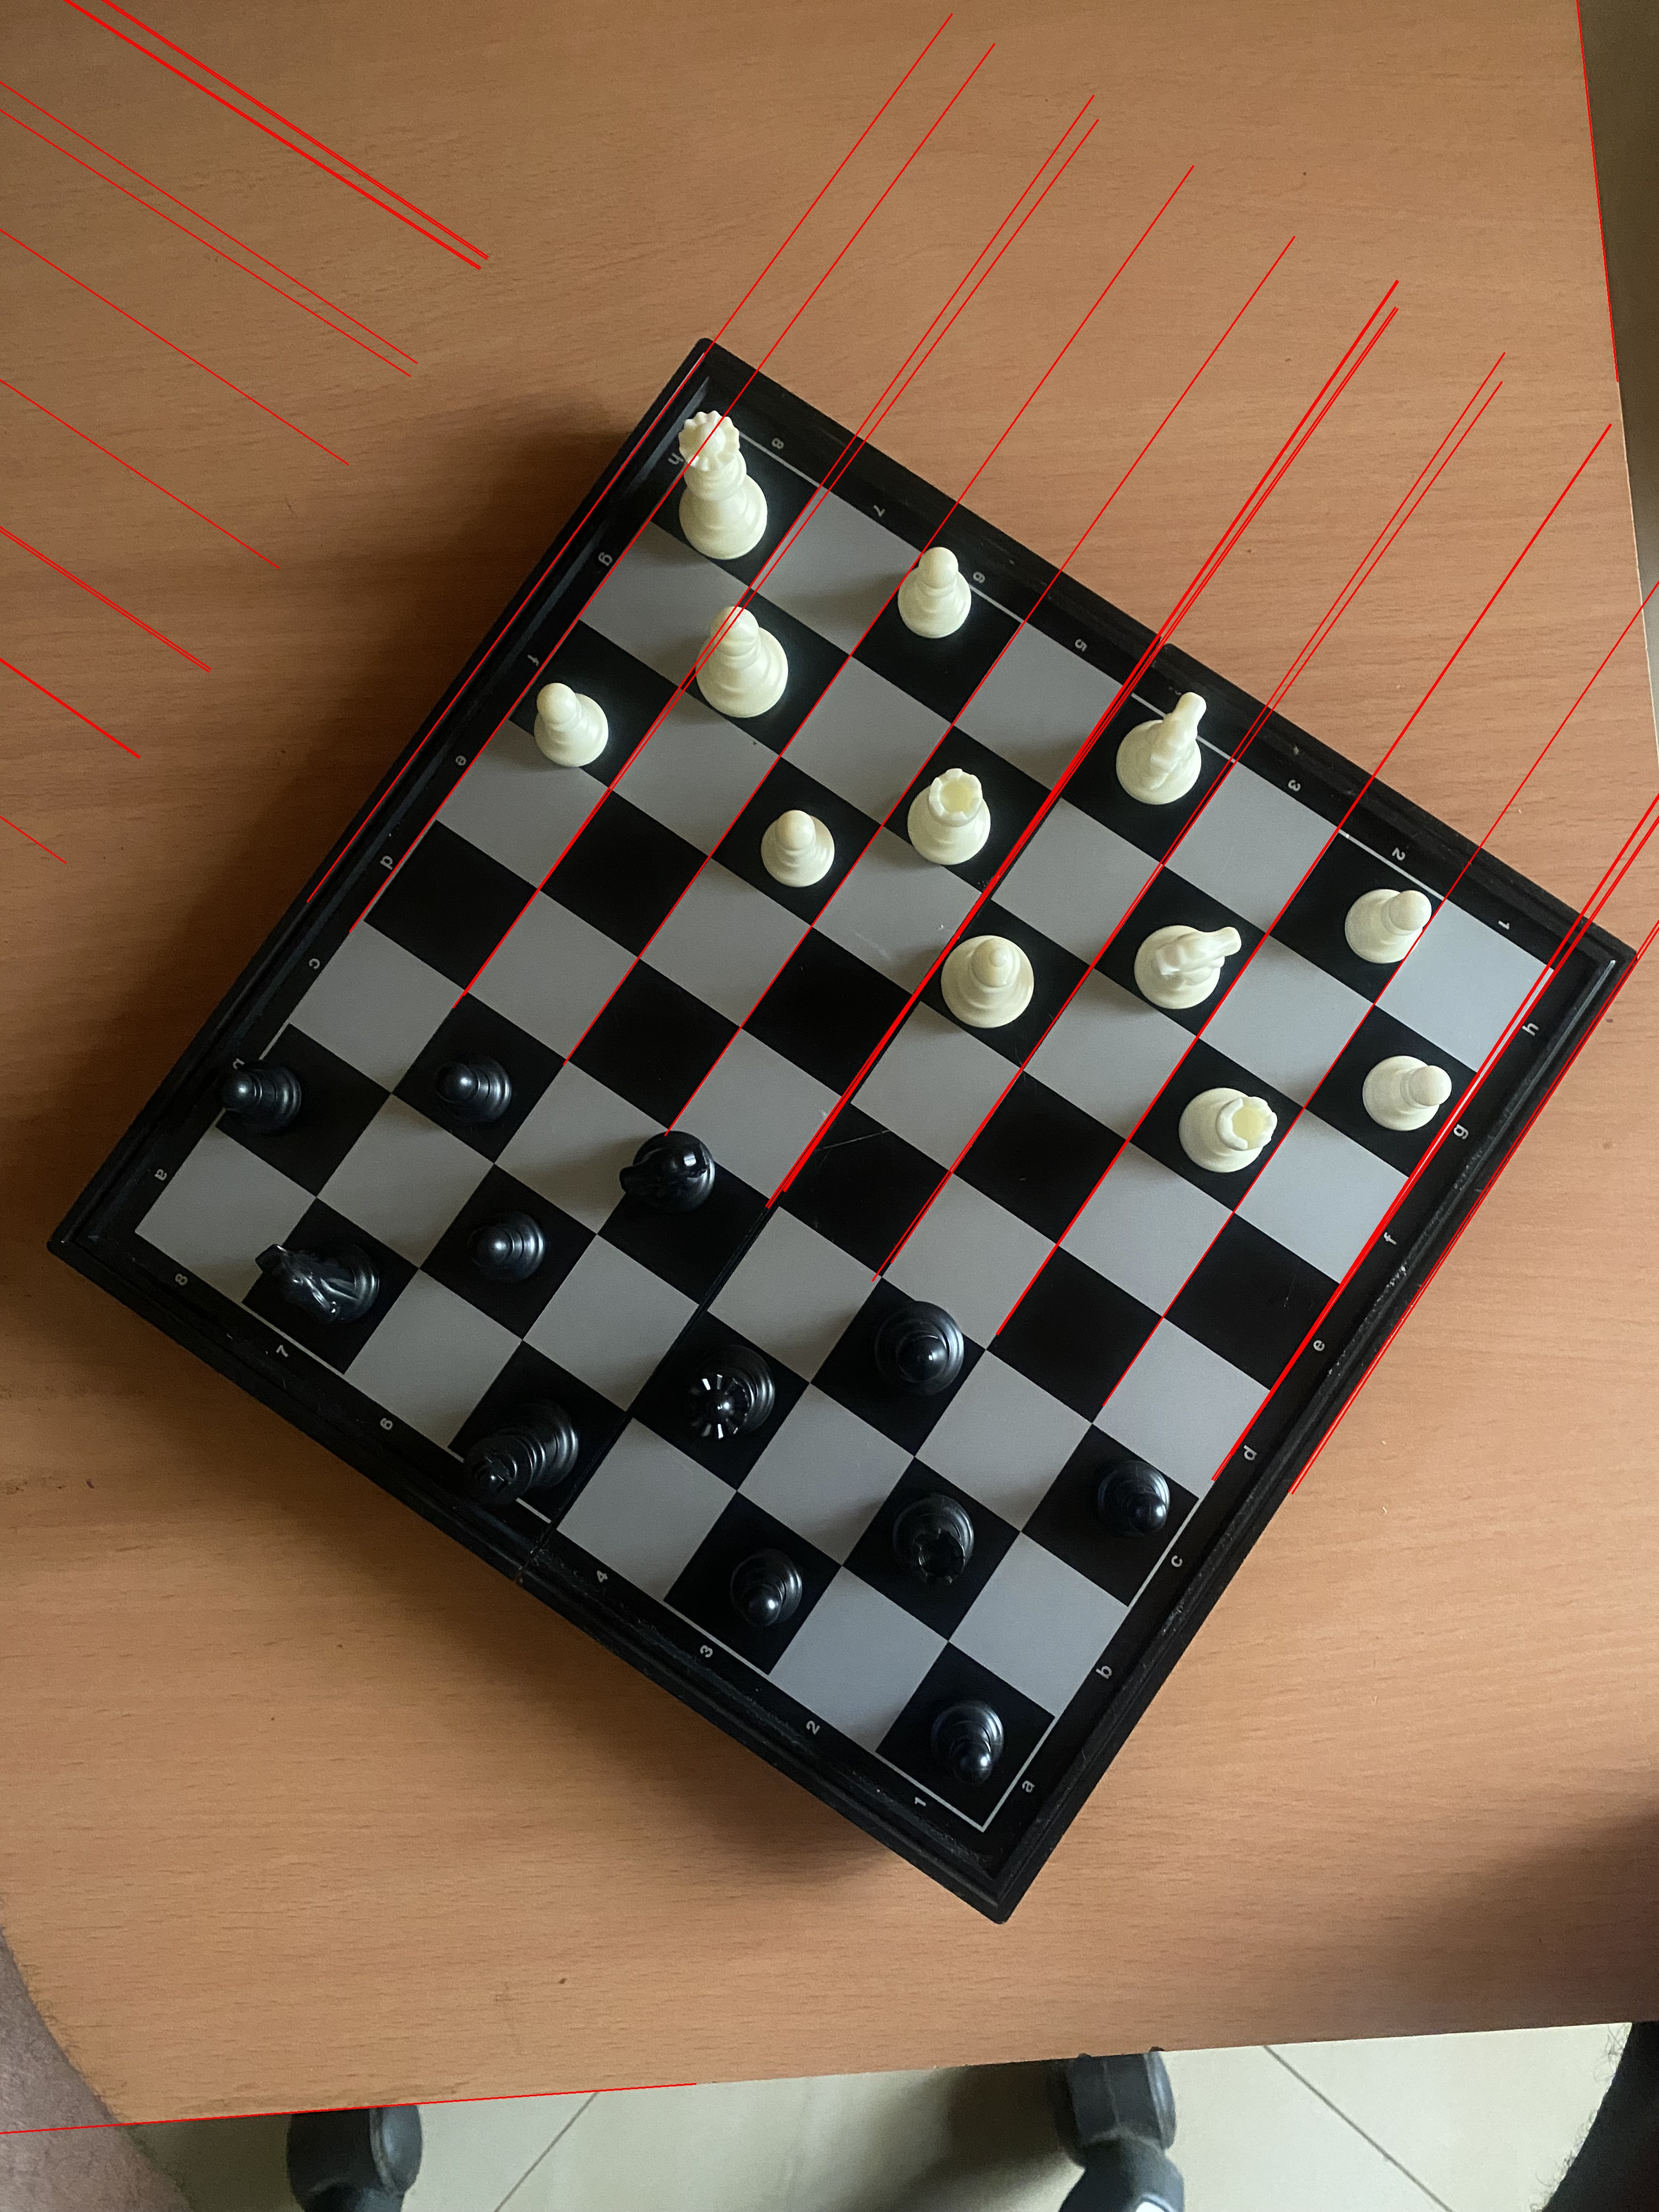
\includegraphics[width=\textwidth]{linesDetected2b.jpg}
        \caption{\texttt{2b} ($34^\circ$)}
    \end{subfigure}
    \hfill
    \begin{subfigure}[b]{0.32\textwidth}
        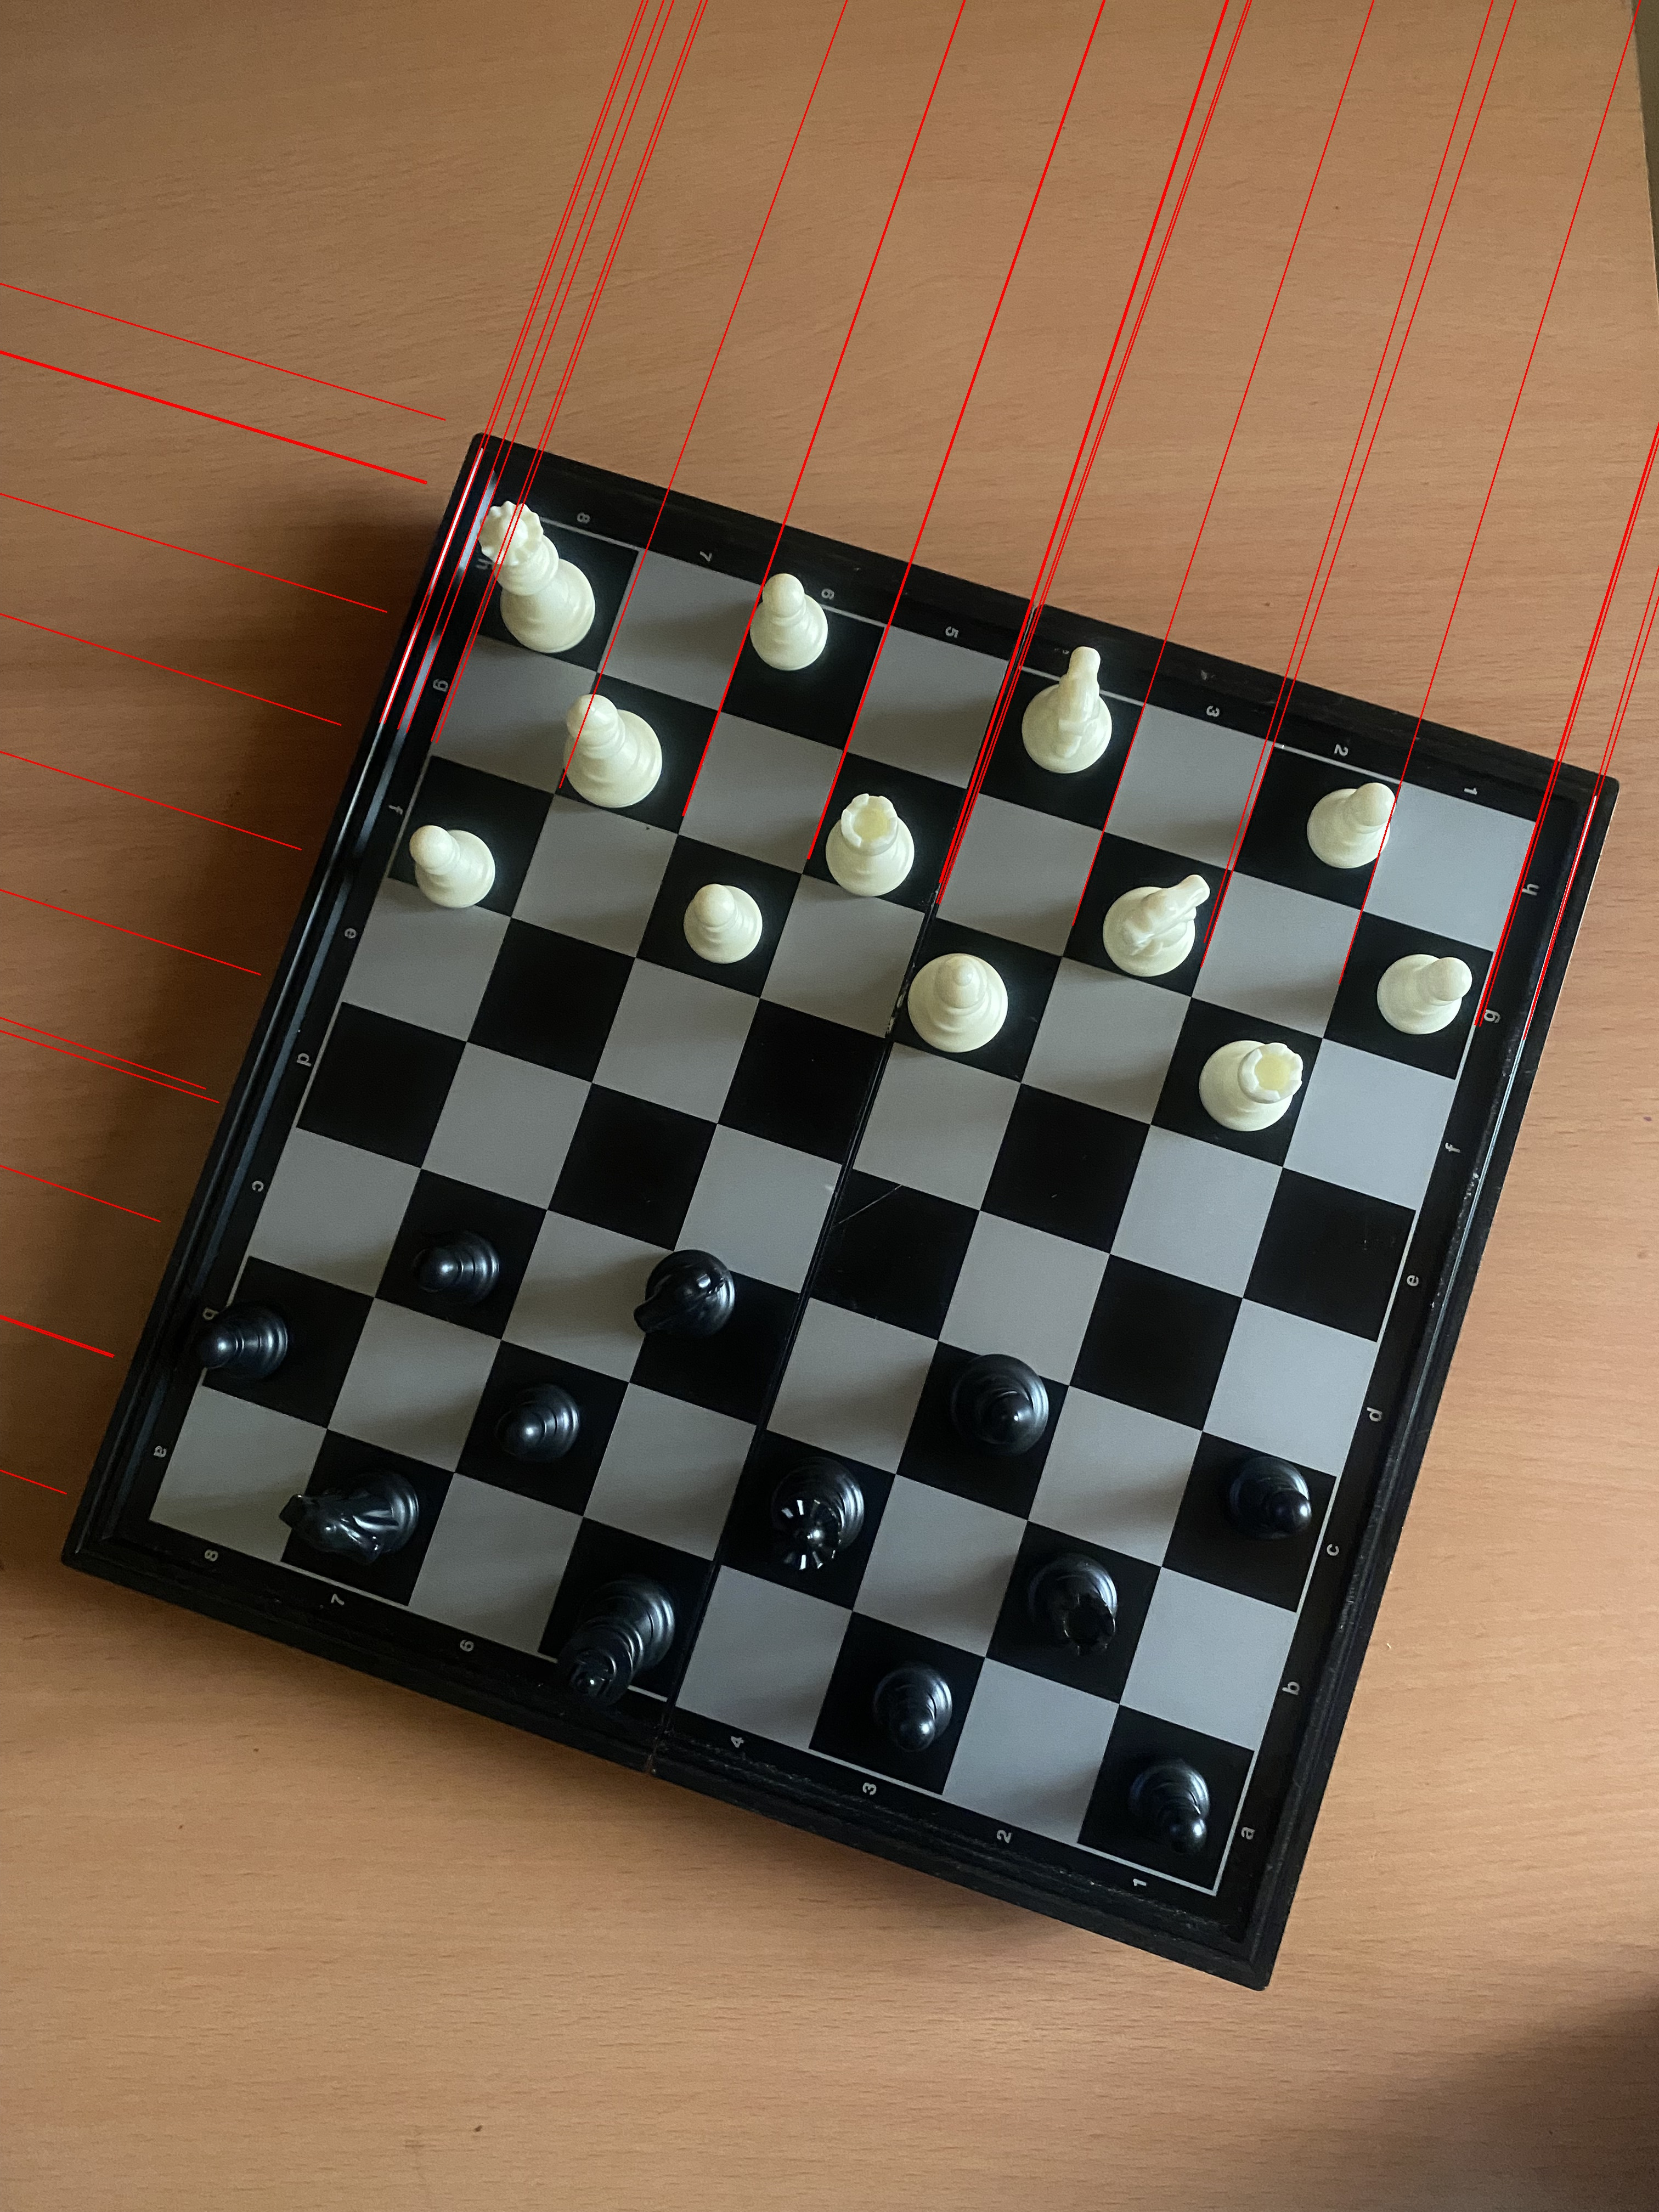
\includegraphics[width=\textwidth]{linesDetected2c.jpg}
        \caption{\texttt{2c} ($20^\circ$)}
    \end{subfigure}
    \caption{Lines detected (red) on each chessboard image using the Hough Transform~\cite{duda1972use}.}
    \label{fig:q2_lines}
\end{figure}

\begin{figure}[H]
    \centering
    \begin{subfigure}[b]{0.32\textwidth}
        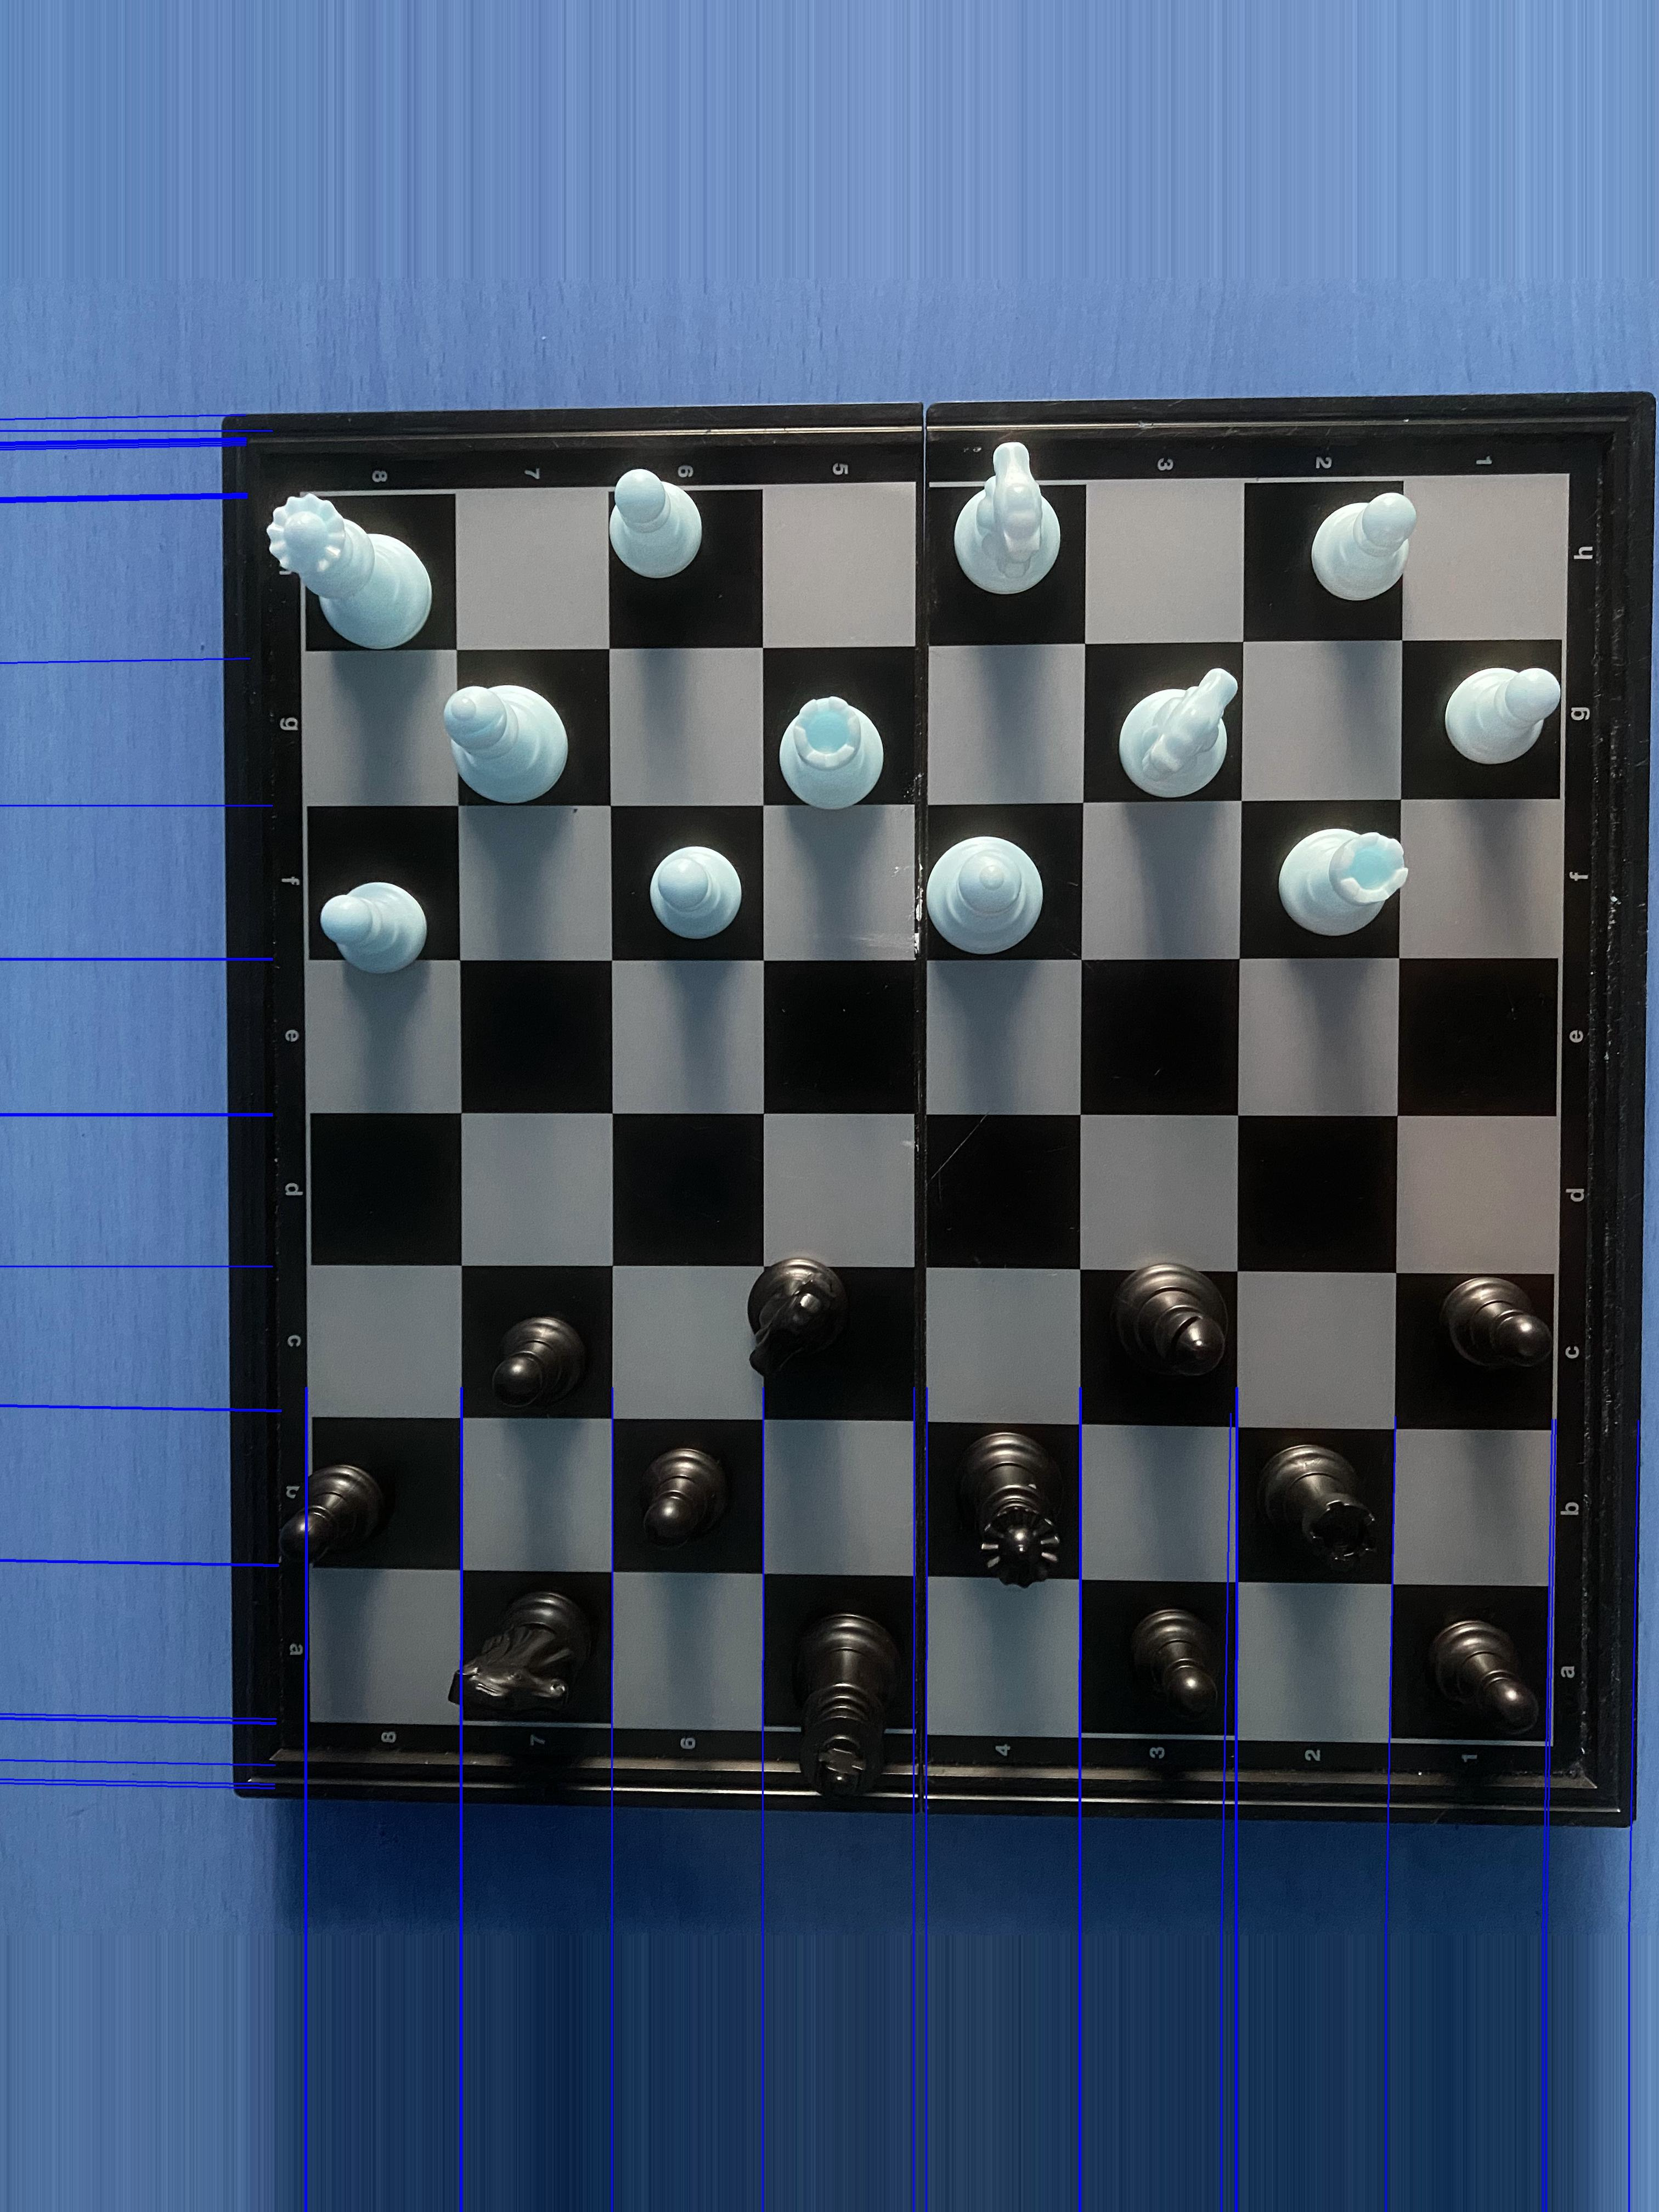
\includegraphics[width=\textwidth]{rotated_image_2a.jpg}
        \caption{\texttt{2a} ($0^\circ$ rotation)}
    \end{subfigure}
    \hfill
    \begin{subfigure}[b]{0.32\textwidth}
        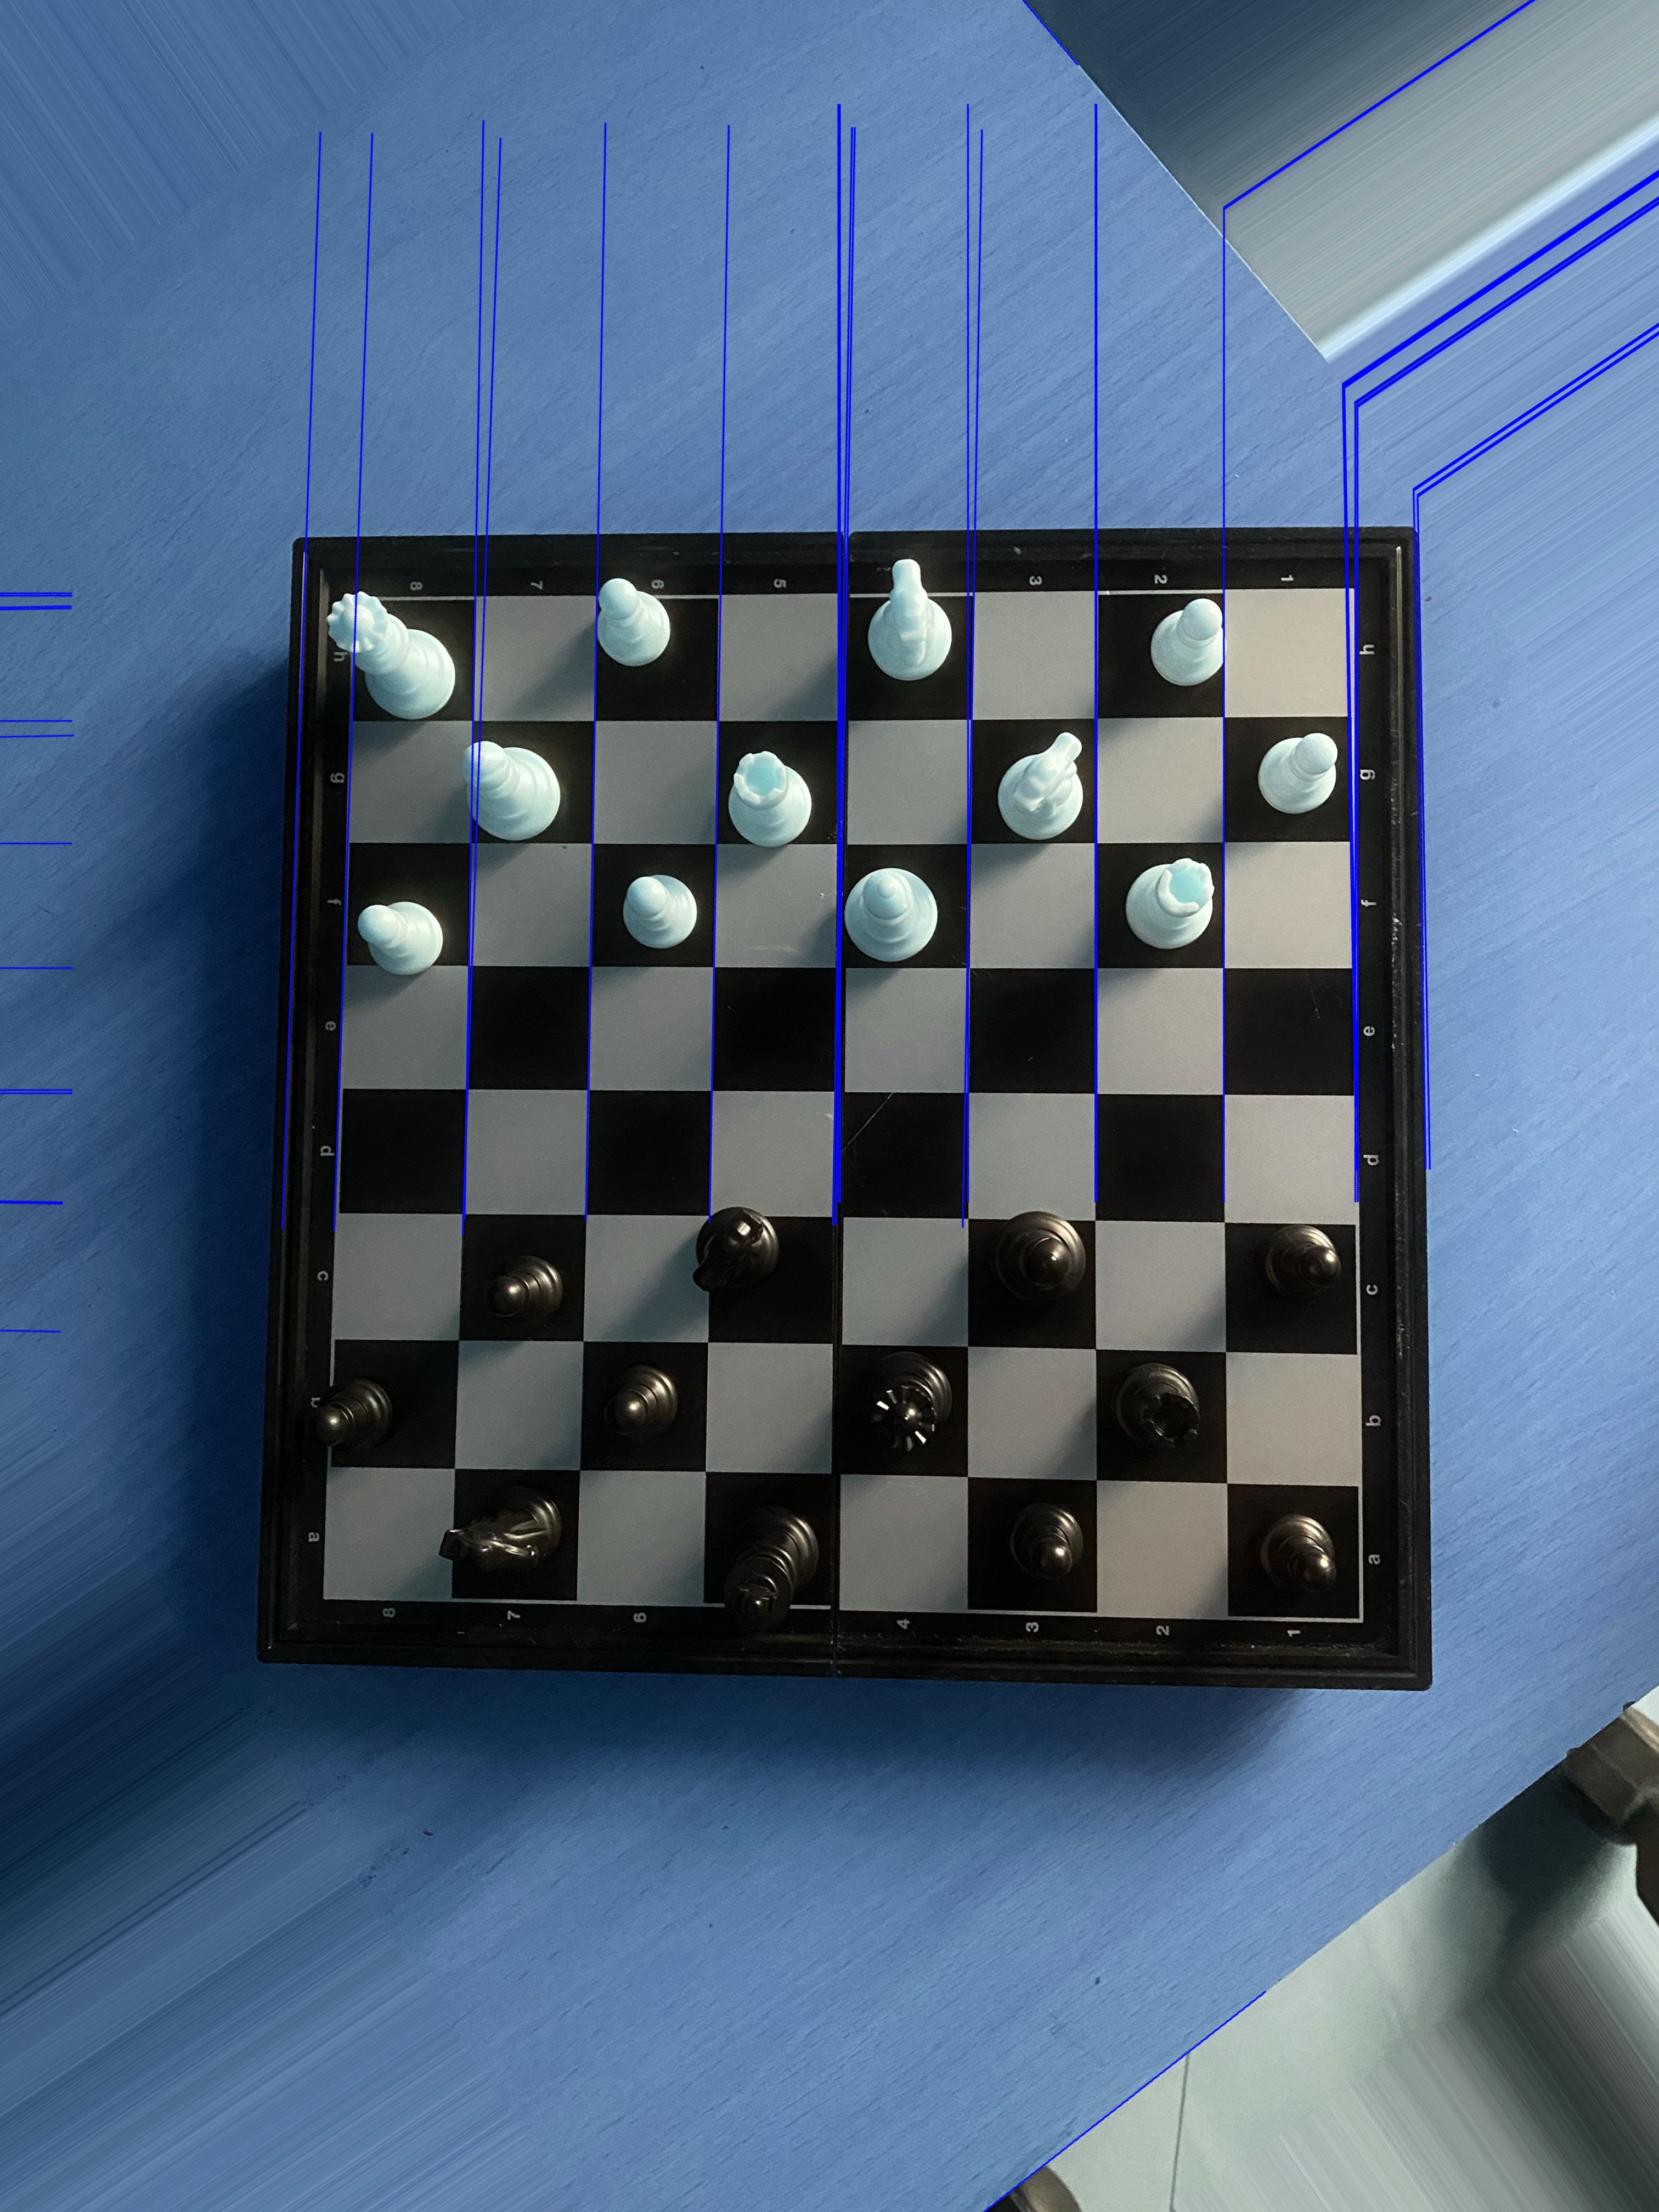
\includegraphics[width=\textwidth]{rotated_image_2b.jpg}
        \caption{\texttt{2b} ($-34^\circ$ rotation)}
    \end{subfigure}
    \hfill
    \begin{subfigure}[b]{0.32\textwidth}
        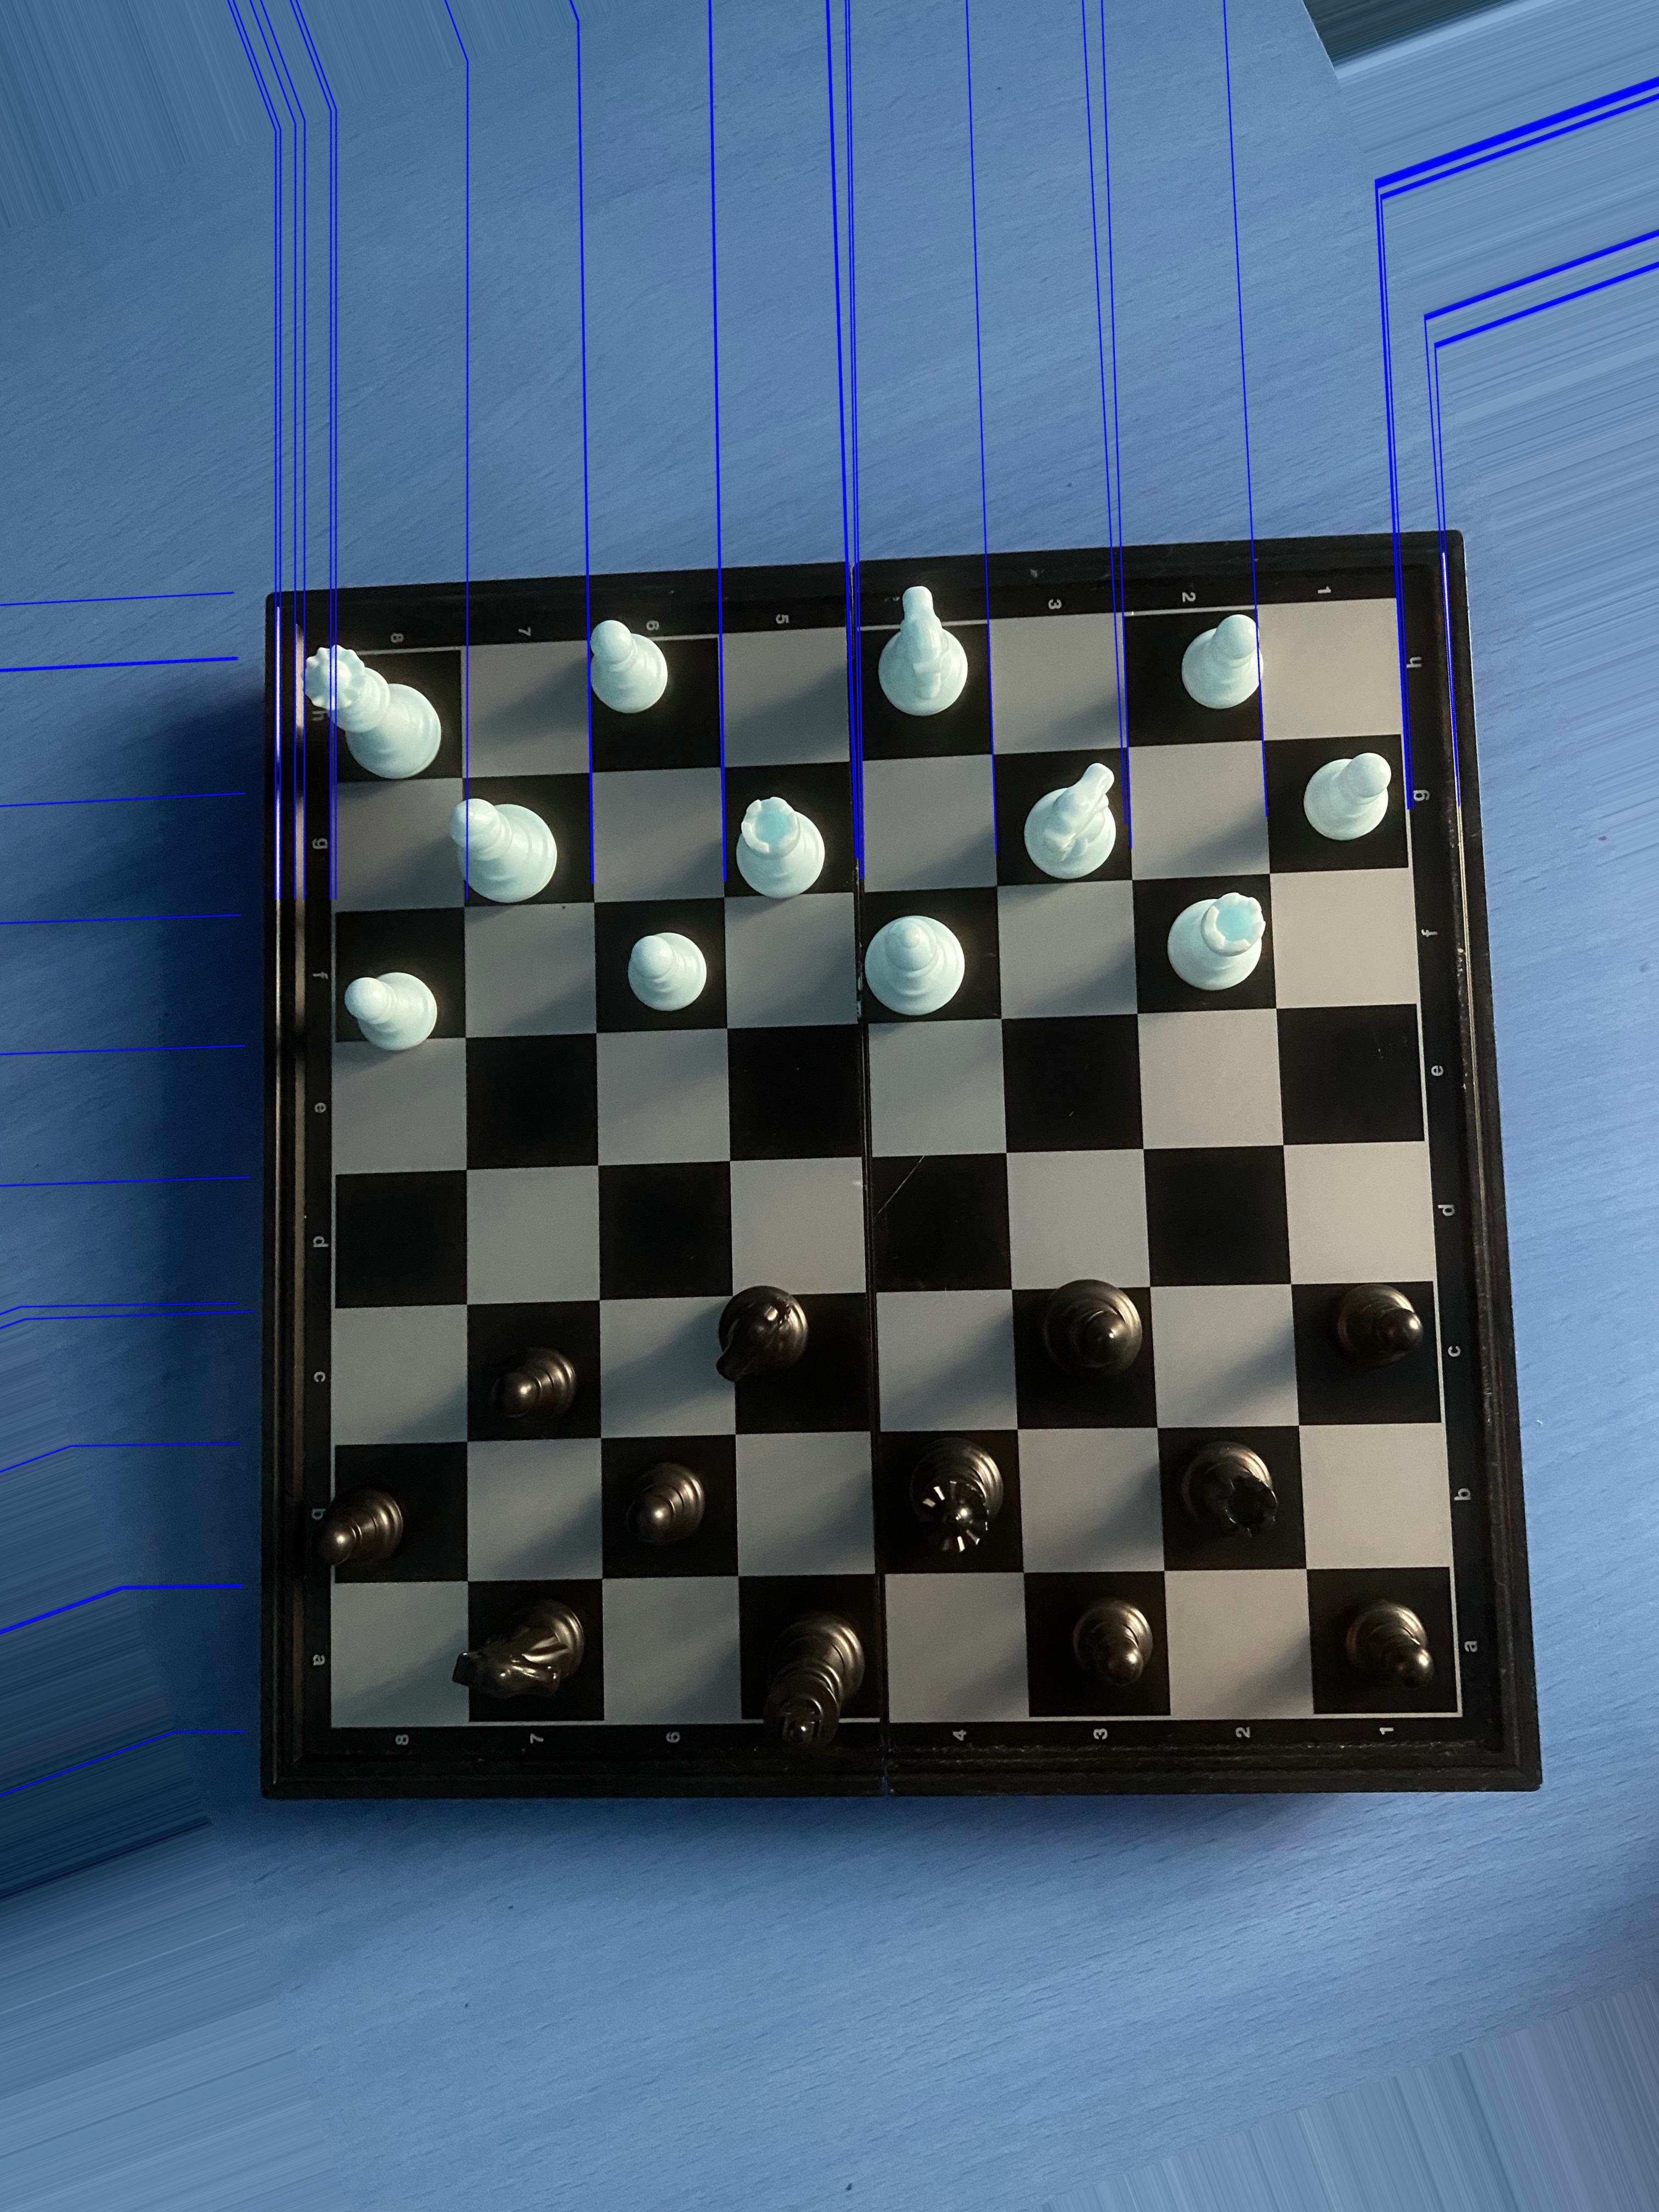
\includegraphics[width=\textwidth]{rotated_image_2c.jpg}
        \caption{\texttt{2c} ($-20^\circ$ rotation)}
    \end{subfigure}
    \caption{Straightened images after applying the computed rotation.}
    \label{fig:q2_straightened}
\end{figure}

\subsection{Real-World Experimentation}
To test the algorithm beyond the provided chessboard images, we photographed a \textbf{Rubik's Cube} (top-down view) tilted at an arbitrary angle. The cube's grid pattern provides strong rectilinear edges similar to a chessboard.

\begin{figure}[H]
    \centering
    \begin{subfigure}[b]{0.45\textwidth}
        
\includegraphics[width=\textwidth]{linesDetectedcube.jpg}
        \caption{Detected lines ($141^\circ$)}
    \end{subfigure}
    \hfill
    \begin{subfigure}[b]{0.45\textwidth}
        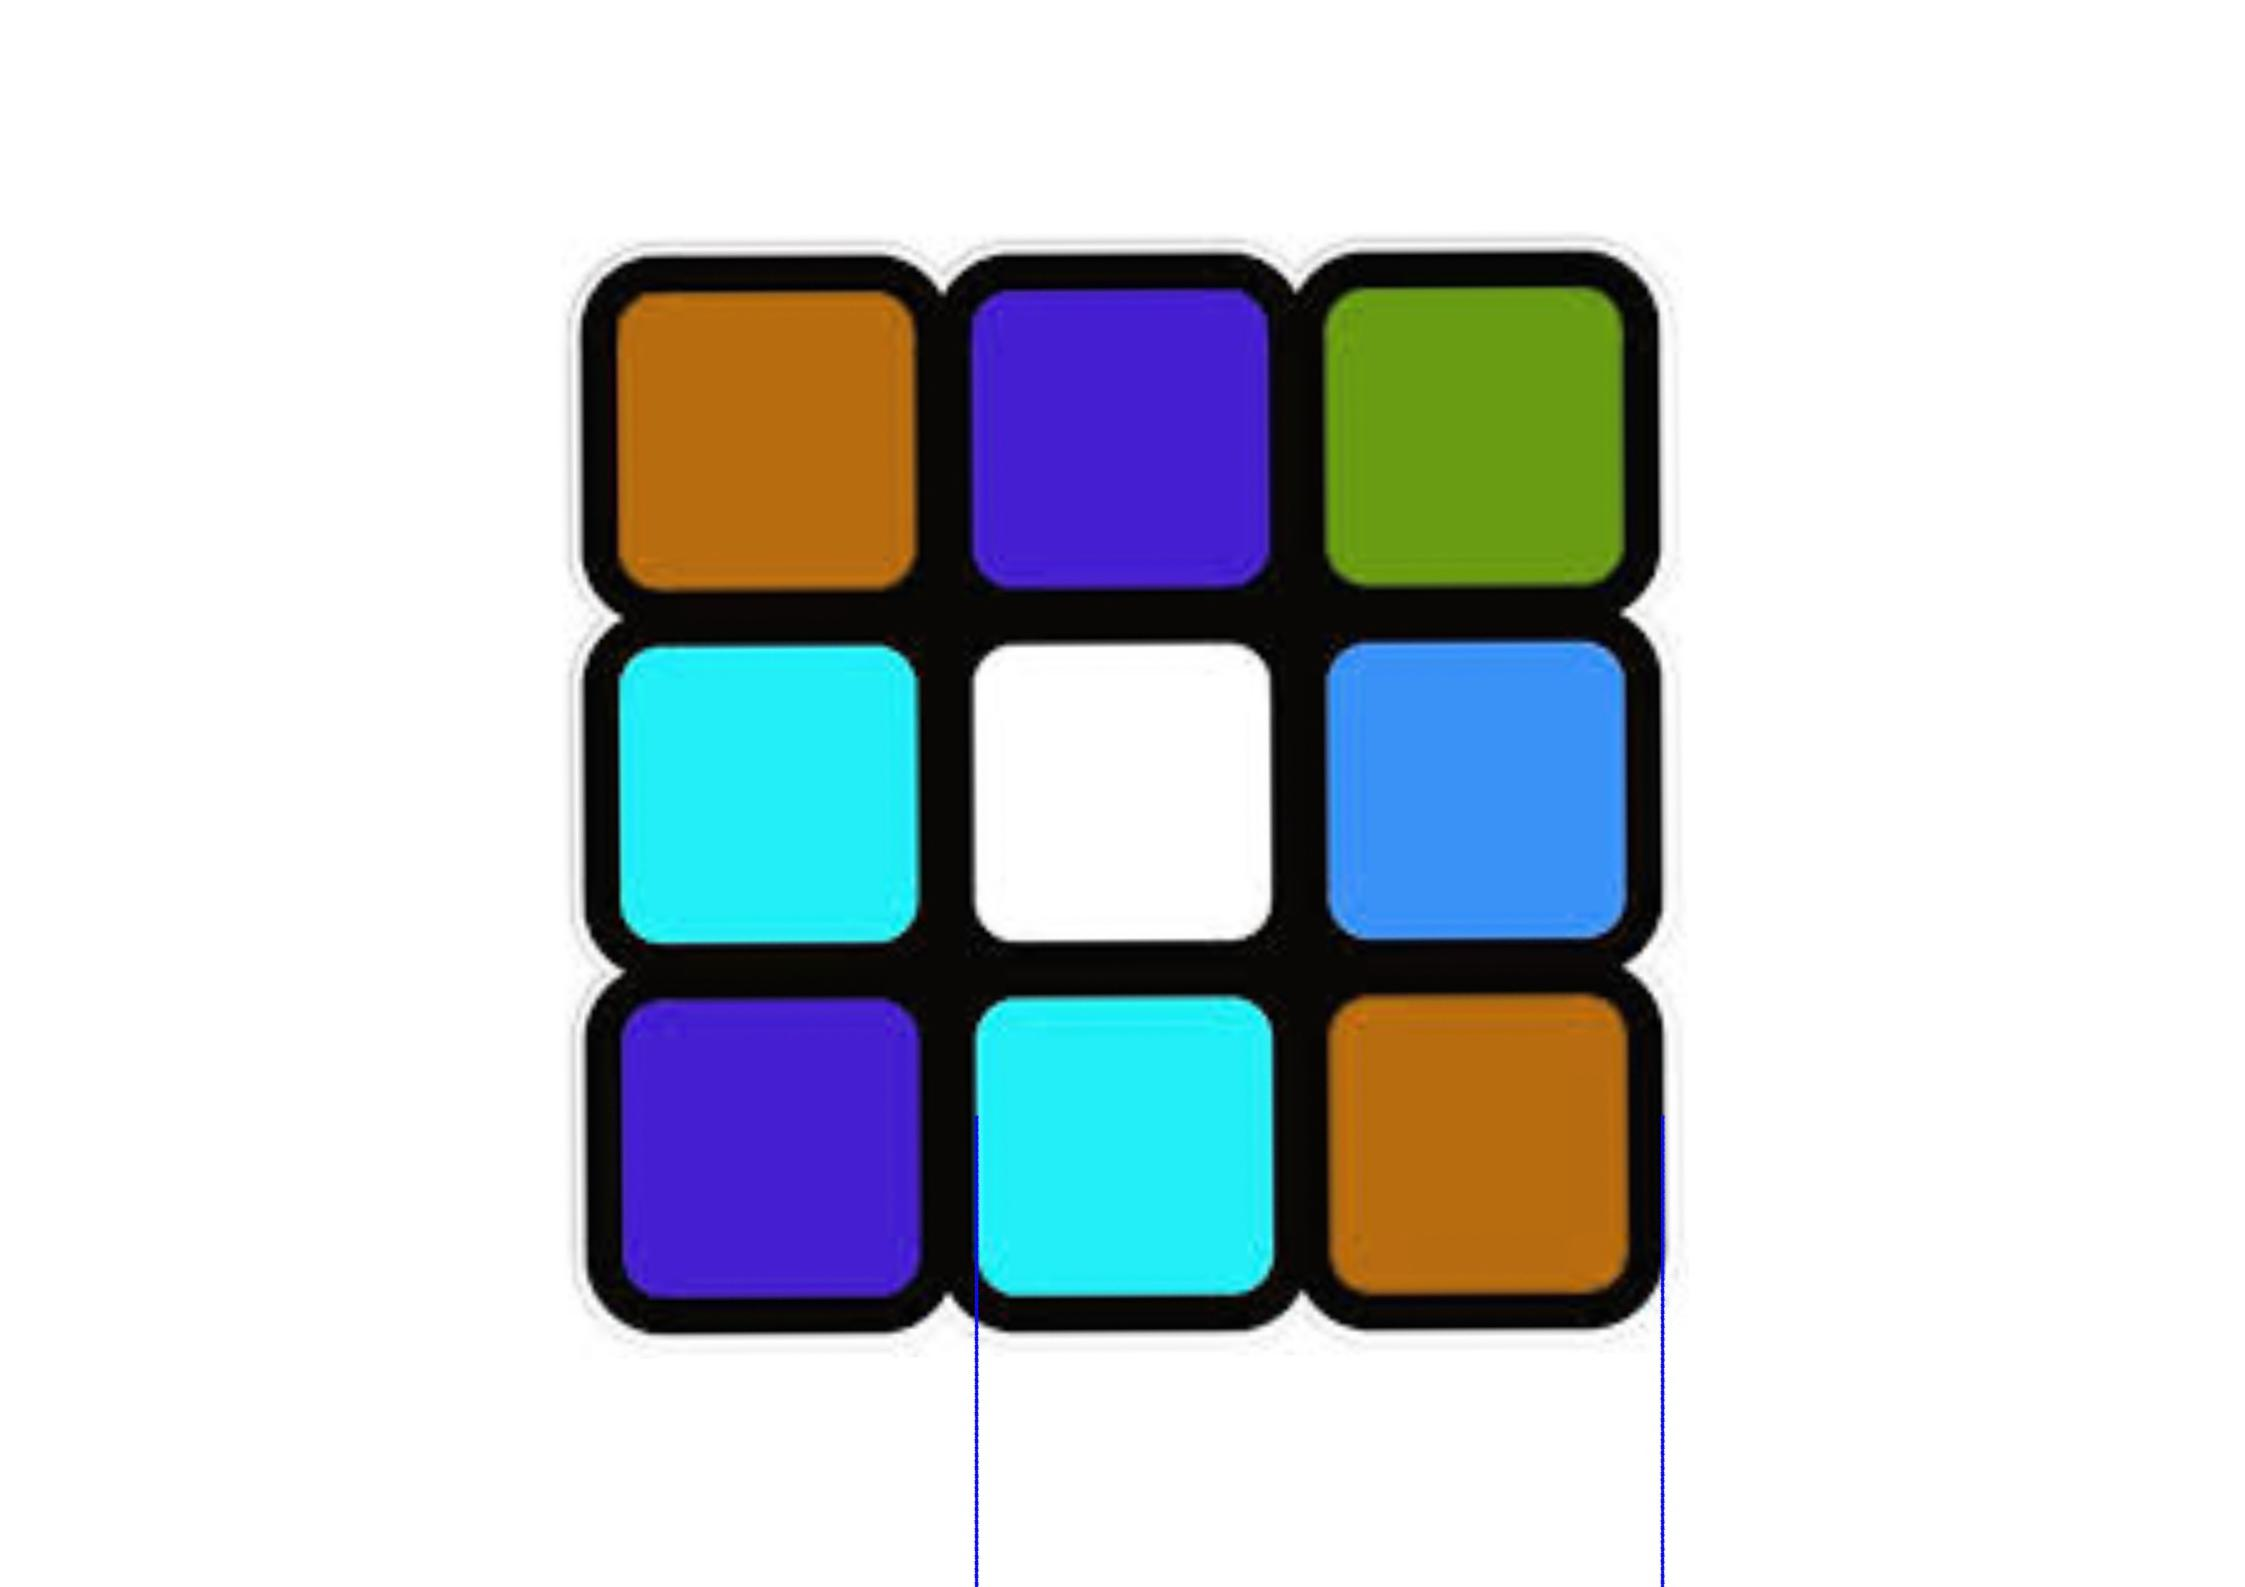
\includegraphics[width=\textwidth]{rotated_image_cube.jpg}
        \caption{Straightened ($39^\circ$ rotation)}
    \end{subfigure}
    \caption{Real-world test: Rubik's Cube top view. The algorithm detects the grid lines and corrects the tilt.}
    \label{fig:q2_realworld}
\end{figure}

The Hough Transform~\cite{duda1972use} successfully detected the cube's grid edges, and the Canny edge detector~\cite{canny1986computational} produced clean edge maps despite the colorful surface. The dominant angle was $141^\circ$, and the algorithm applied a $39^\circ$ rotation to align the grid.

\textit{Note: In Figure~\ref{fig:q2_realworld}, a noticeable color shift (e.g., red/blue inversion) is observed between the original and straightened images. This artifact arises because OpenCV loads images in BGR format, while the visualization library (Matplotlib) expects RGB. This purely visual discrepancy does not affect the geometric transformation, as the algorithm operates on the single-channel grayscale intensity.}

\subsection{Difficulties of the Naive Straightening Algorithm}
While our pipeline works well for structured grids, several limitations were observed:

\begin{enumerate}
    \item \textbf{Ambiguous dominant direction:} When an image contains equally strong lines in multiple orientations (e.g., both horizontal and vertical), the dominant angle from vote counting may be arbitrary. The algorithm assumes one dominant direction, which can fail for symmetric objects.

    \item \textbf{Sensitivity to threshold tuning:} The Hough Transform threshold must be carefully tuned per image. A value optimized for the chessboard (300) was too high for the Rubik's Cube, which required a lower threshold (150). There is no universal threshold.

    \item \textbf{Non-rectilinear structures:} The algorithm snaps to the nearest cardinal axis ($0^\circ$, $90^\circ$, $180^\circ$). For objects intentionally at $45^\circ$ (e.g., a diamond shape), the algorithm would incorrectly ``correct'' a valid orientation.

    \item \textbf{Border artifacts:} After rotation, image corners contain regions outside the original frame. Using \texttt{cv2.BORDER\_REPLICATE} fills these with edge pixels, which can create visual artifacts. Cropping to the largest inscribed rectangle would solve this but reduces the field of view.
\end{enumerate}

\subsection{Other Real-World Scenarios for Image Alignment}
Automatic image straightening is valuable in many domains:

\begin{enumerate}
    \item \textbf{Document scanning and OCR:} Scanned documents or phone-captured text are often tilted. Straightening (deskewing) improves OCR accuracy significantly, as most engines assume horizontal text~\cite{das2001deskewing}.

    \item \textbf{Satellite and aerial imagery:} Aligning satellite images to a north-up orientation is essential for map overlays, change detection, and urban planning~\cite{opencv_docs}.

    \item \textbf{Medical imaging:} X-rays, MRIs, and CT scans must be consistently aligned for diagnosis comparison and automated analysis~\cite{oliveira2014medical}.

    \item \textbf{Autonomous driving:} Lane detection requires identifying road lines and correcting for camera tilt to produce reliable heading estimates~\cite{hillel2014lanes}.

    \item \textbf{Architectural photography:} Correcting perspective distortion in building photographs to ensure vertical lines remain vertical (keystone correction).
\end{enumerate}

\newpage
\section{Image Compression with Fourier Transform}

\subsection{Goal}
The goal of this section is to implement a lossy image compression algorithm using the Fast Fourier Transform (FFT). We aim to reduce the data size of high-resolution satellite imagery while preserving essential geographic features (coastlines, roads) by filtering out less significant frequency components.

\subsection{Methodology}
The fundamental principle of Fourier-based compression is that most of the "energy" (visual information) in a natural image is concentrated in the low-frequency components. By transforming the image to the frequency domain, we can keep only the coefficients with the highest magnitudes and discard the rest.

\subsubsection{Discrete Fourier Transform (DFT)}
For an image $f(x,y)$ of size $M \times N$, the 2D DFT ~\cite{park20152d} is defined as:
\begin{equation}
    F(u,v) = \sum_{x=0}^{M-1} \sum_{y=0}^{N-1} f(x,y) e^{-j 2\pi (ux/M + vy/N)}
\end{equation}
where $F(u,v)$ is the complex frequency spectrum. The magnitude spectrum $|F(u,v)|$ indicates the strength of each frequency.

\subsubsection{Compression Algorithm}
We implemented the following pipeline:
\begin{enumerate}
    \item \textbf{FFT Computation:} Compute the 2D FFT of the grayscale image and shift the zero-frequency component to the center.
    \item \textbf{Thresholding:} Calculate the magnitude of all frequency coefficients. We apply a ``hard threshold'' where we retain only the top $k\%$ of coefficients (e.g., $10\%$) with the largest magnitudes. All other coefficients are set to zero.
    \item \textbf{Reconstruction:} Apply the Inverse FFT (IFFT) to the filtered spectrum to recover the spatial domain image.
\end{enumerate}

\subsection{Results}
We tested the algorithm on two distinct images from the \texttt{q3\_data} dataset:
\begin{itemize}
    \item \textbf{High-Frequency Image (\texttt{q3a.jpg}):} A high-resolution satellite image rich in texture and edges.
    \item \textbf{Low-Frequency Image (\texttt{q3b.jpg}):} A simpler image with smoother transitions.
\end{itemize}

\begin{figure}[!ht]
    \centering
    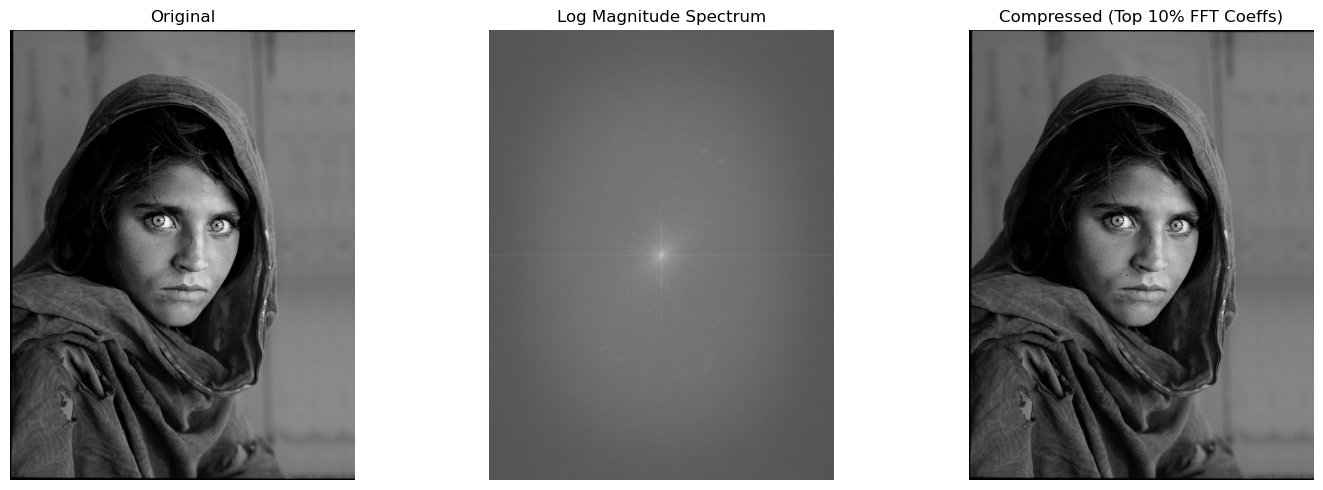
\includegraphics[width=0.9\textwidth]{comparison_q3a.png}
    \caption{Compression results for the high-resolution satellite image (\texttt{q3a.jpg}). Left: Original. Center: Log-Magnitude Spectrum. Right: Compressed image retaining top 10\% of coefficients.}
    \label{fig:q3_satellite}
\end{figure}

\begin{figure}[!ht]
    \centering
    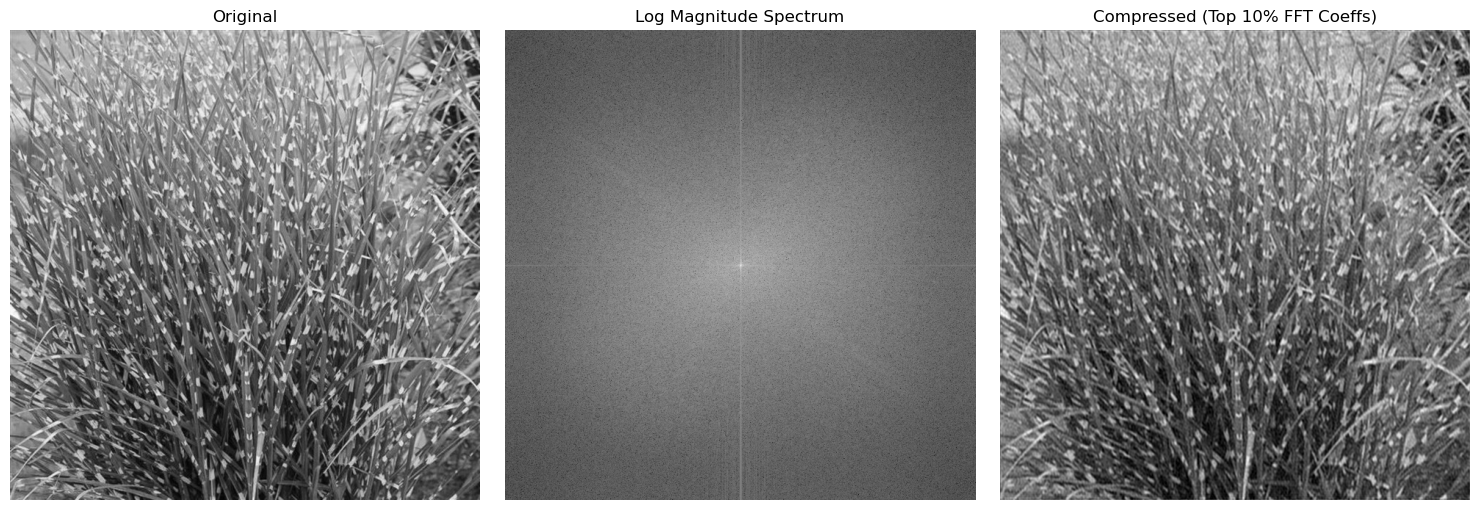
\includegraphics[width=0.9\textwidth]{comparison_q3b.png}
    \caption{Compression results for the low-frequency image (\texttt{q3b.jpg}). The compressed version retains high fidelity even with significant data removal.}
    \label{fig:q3_lowfreq}
\end{figure}

\begin{figure}[!ht]
    \centering
    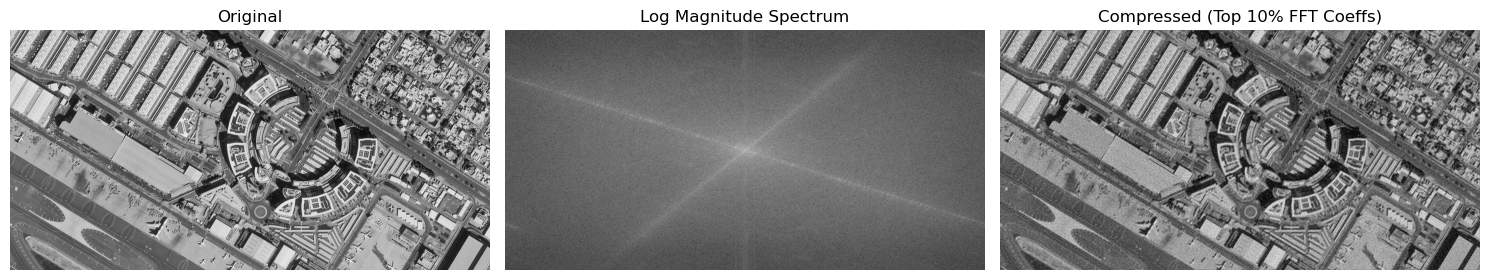
\includegraphics[width=0.9\textwidth]{comparison_sat_img1.png}
    \caption{Compression results for the newly acquired satellite image (\texttt{sat\_img1.jpg}). The algorithm preserves large-scale features while achieving compression.}
    \label{fig:q3_sat_img1}
\end{figure}

\subsubsection{Observations}
\begin{itemize}
    \item \textbf{Satellite Image:} The compressed image successfully preserves major structural features like coastlines and roads. However, filtering out high frequencies introduces ``ringing'' artifacts (Gibbs phenomenon~\cite{gonzalez2018digital}) around sharp edges and blurs fine texture (e.g., waves or vegetation).
    \item \textbf{Compression Rate:} By retaining only $10\%$ of the coefficients, we theoretically achieve a significant reduction in data size, though the actual file size depends on the encoding of the sparse matrix.
\end{itemize}

\newpage
\section{Data Augmentation}

\subsection{Methodology}
Data augmentation increases dataset diversity to improve model robustness~\cite{shorten2019survey}. We implemented five types of augmentations:
\begin{itemize}
    \item \textbf{Resizing:} Scaling images to $224 \times 224$ using Nearest Neighbor (fast, blocky) and Bicubic (smooth) interpolation.
    \item \textbf{Flipping:} Mirroring images horizontally (left-right) and vertically (up-down).
    \item \textbf{Blur/Noise:} Applying Gaussian Blur to simulate focus issues.
    \item \textbf{Rotation:} Rotating the image by $30^\circ$ using an affine transform.
    \item \textbf{Shear:} Applying a shear transformation along the X and Y axes to simulate perspective shifts~\cite{simard2003best}.
\end{itemize}

\subsection{Results}
We applied these augmentations to the chessboard image (\texttt{2a.jpg}). The results are shown in Figure~\ref{fig:q4_results}.

\begin{figure}[!ht]
    \centering
    \begin{subfigure}[b]{0.19\textwidth}
        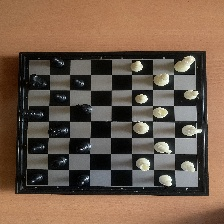
\includegraphics[width=\linewidth]{q4_resize1.jpg}
        \caption{Resize (Nearest)}
    \end{subfigure}
    \hfill
    \begin{subfigure}[b]{0.19\textwidth}
        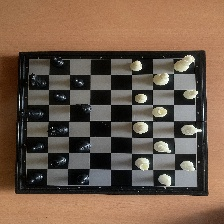
\includegraphics[width=\linewidth]{q4_resize2.jpg}
        \caption{Resize (Bicubic)}
    \end{subfigure}
    \hfill
    \begin{subfigure}[b]{0.19\textwidth}
        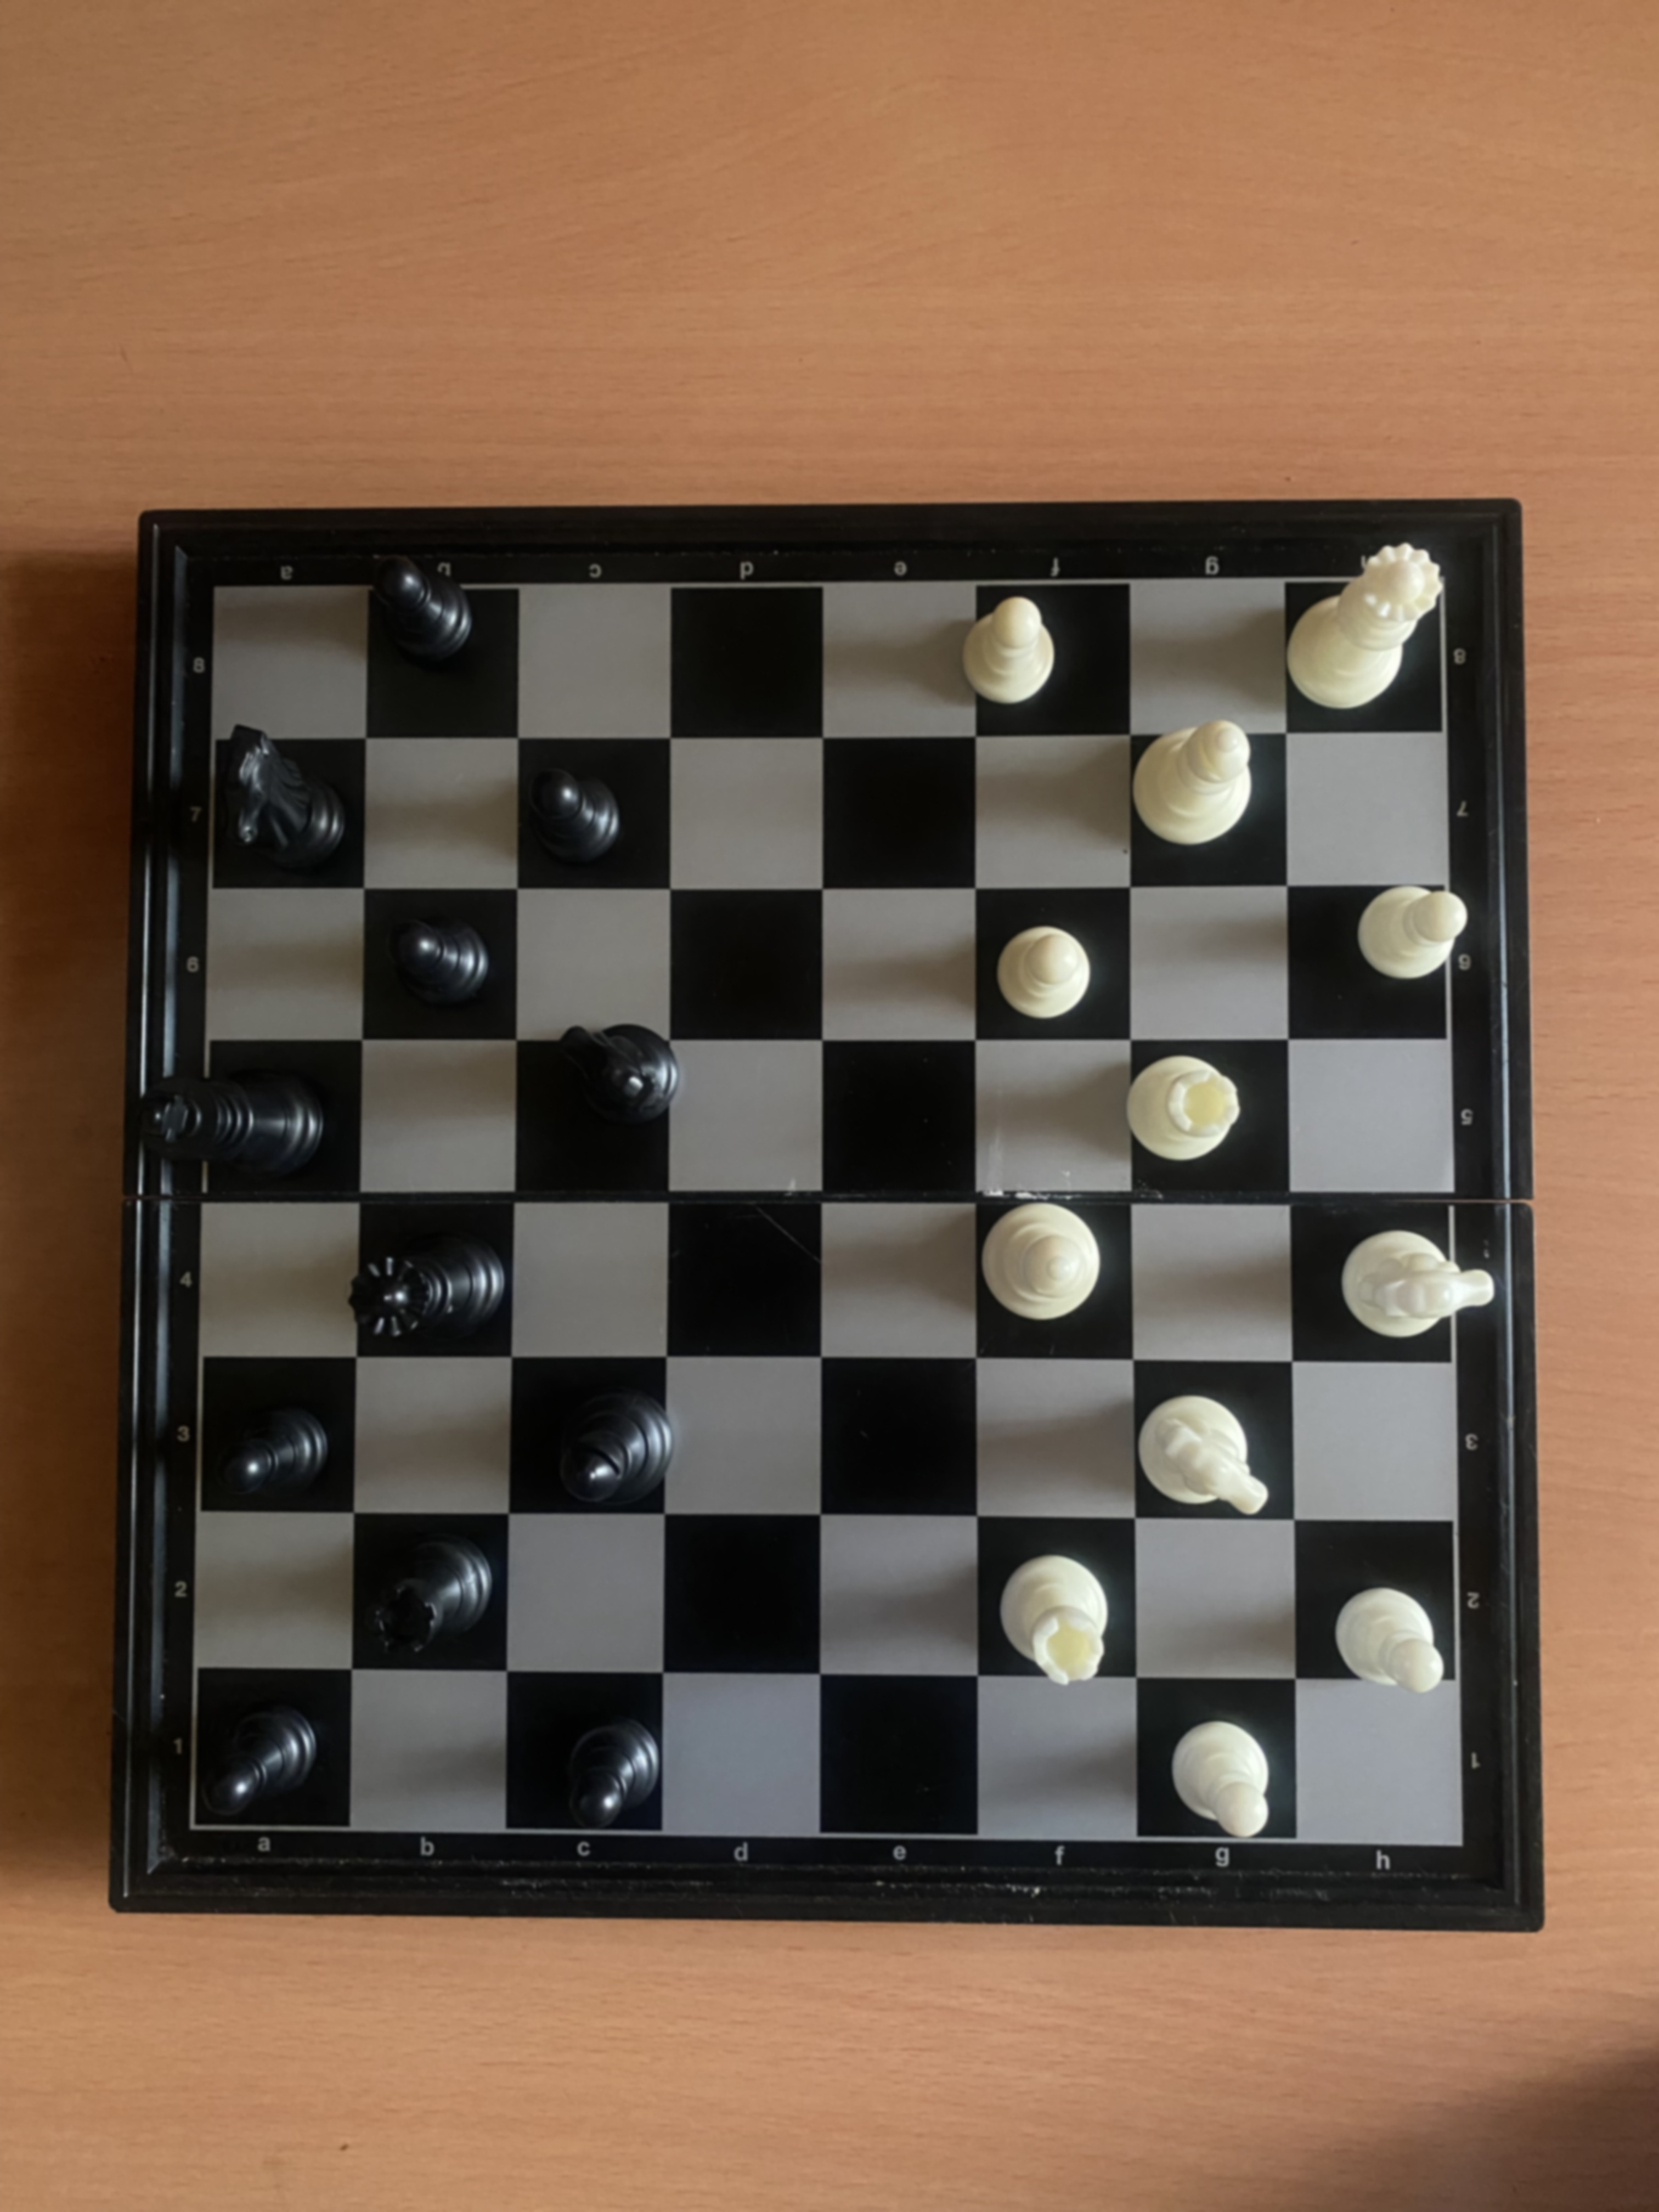
\includegraphics[width=\linewidth]{q4_blur_noise.jpg}
        \caption{Gaussian Blur}
    \end{subfigure}
    \hfill
    \begin{subfigure}[b]{0.19\textwidth}
        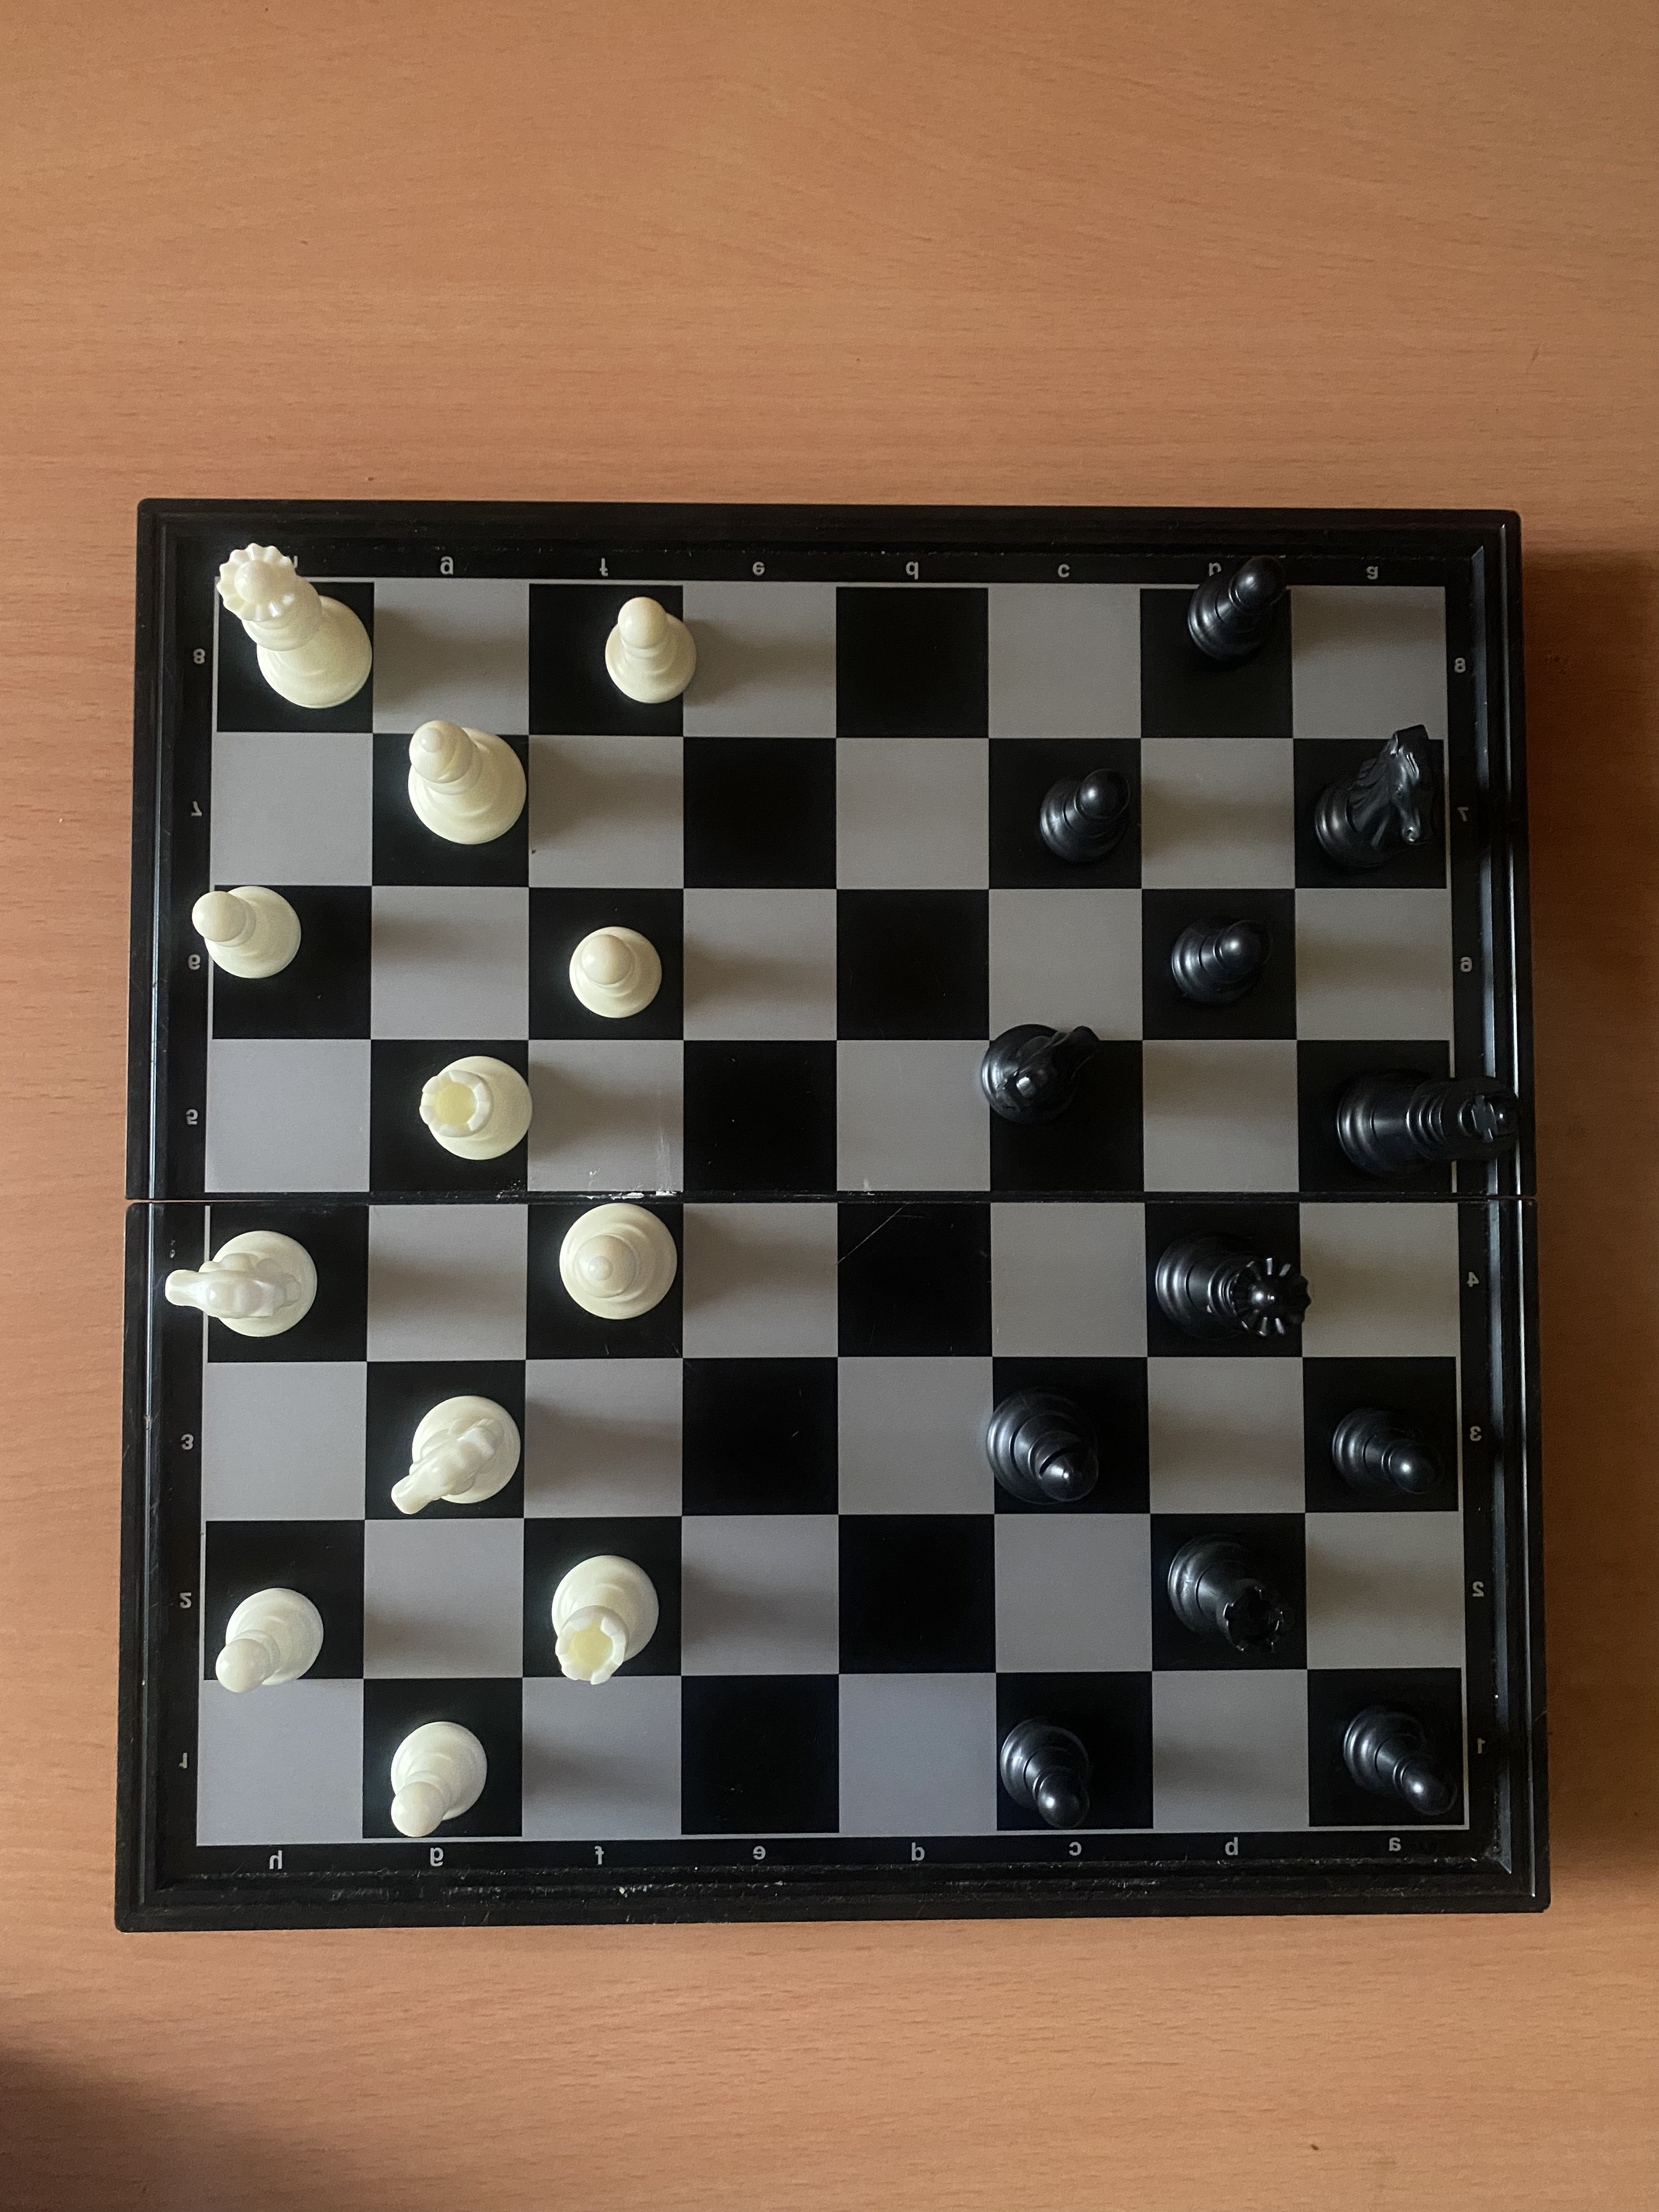
\includegraphics[width=\linewidth]{q4_horizontal_flip.jpg}
        \caption{H-Flip}
    \end{subfigure}
    
    \begin{subfigure}[b]{0.19\textwidth}
        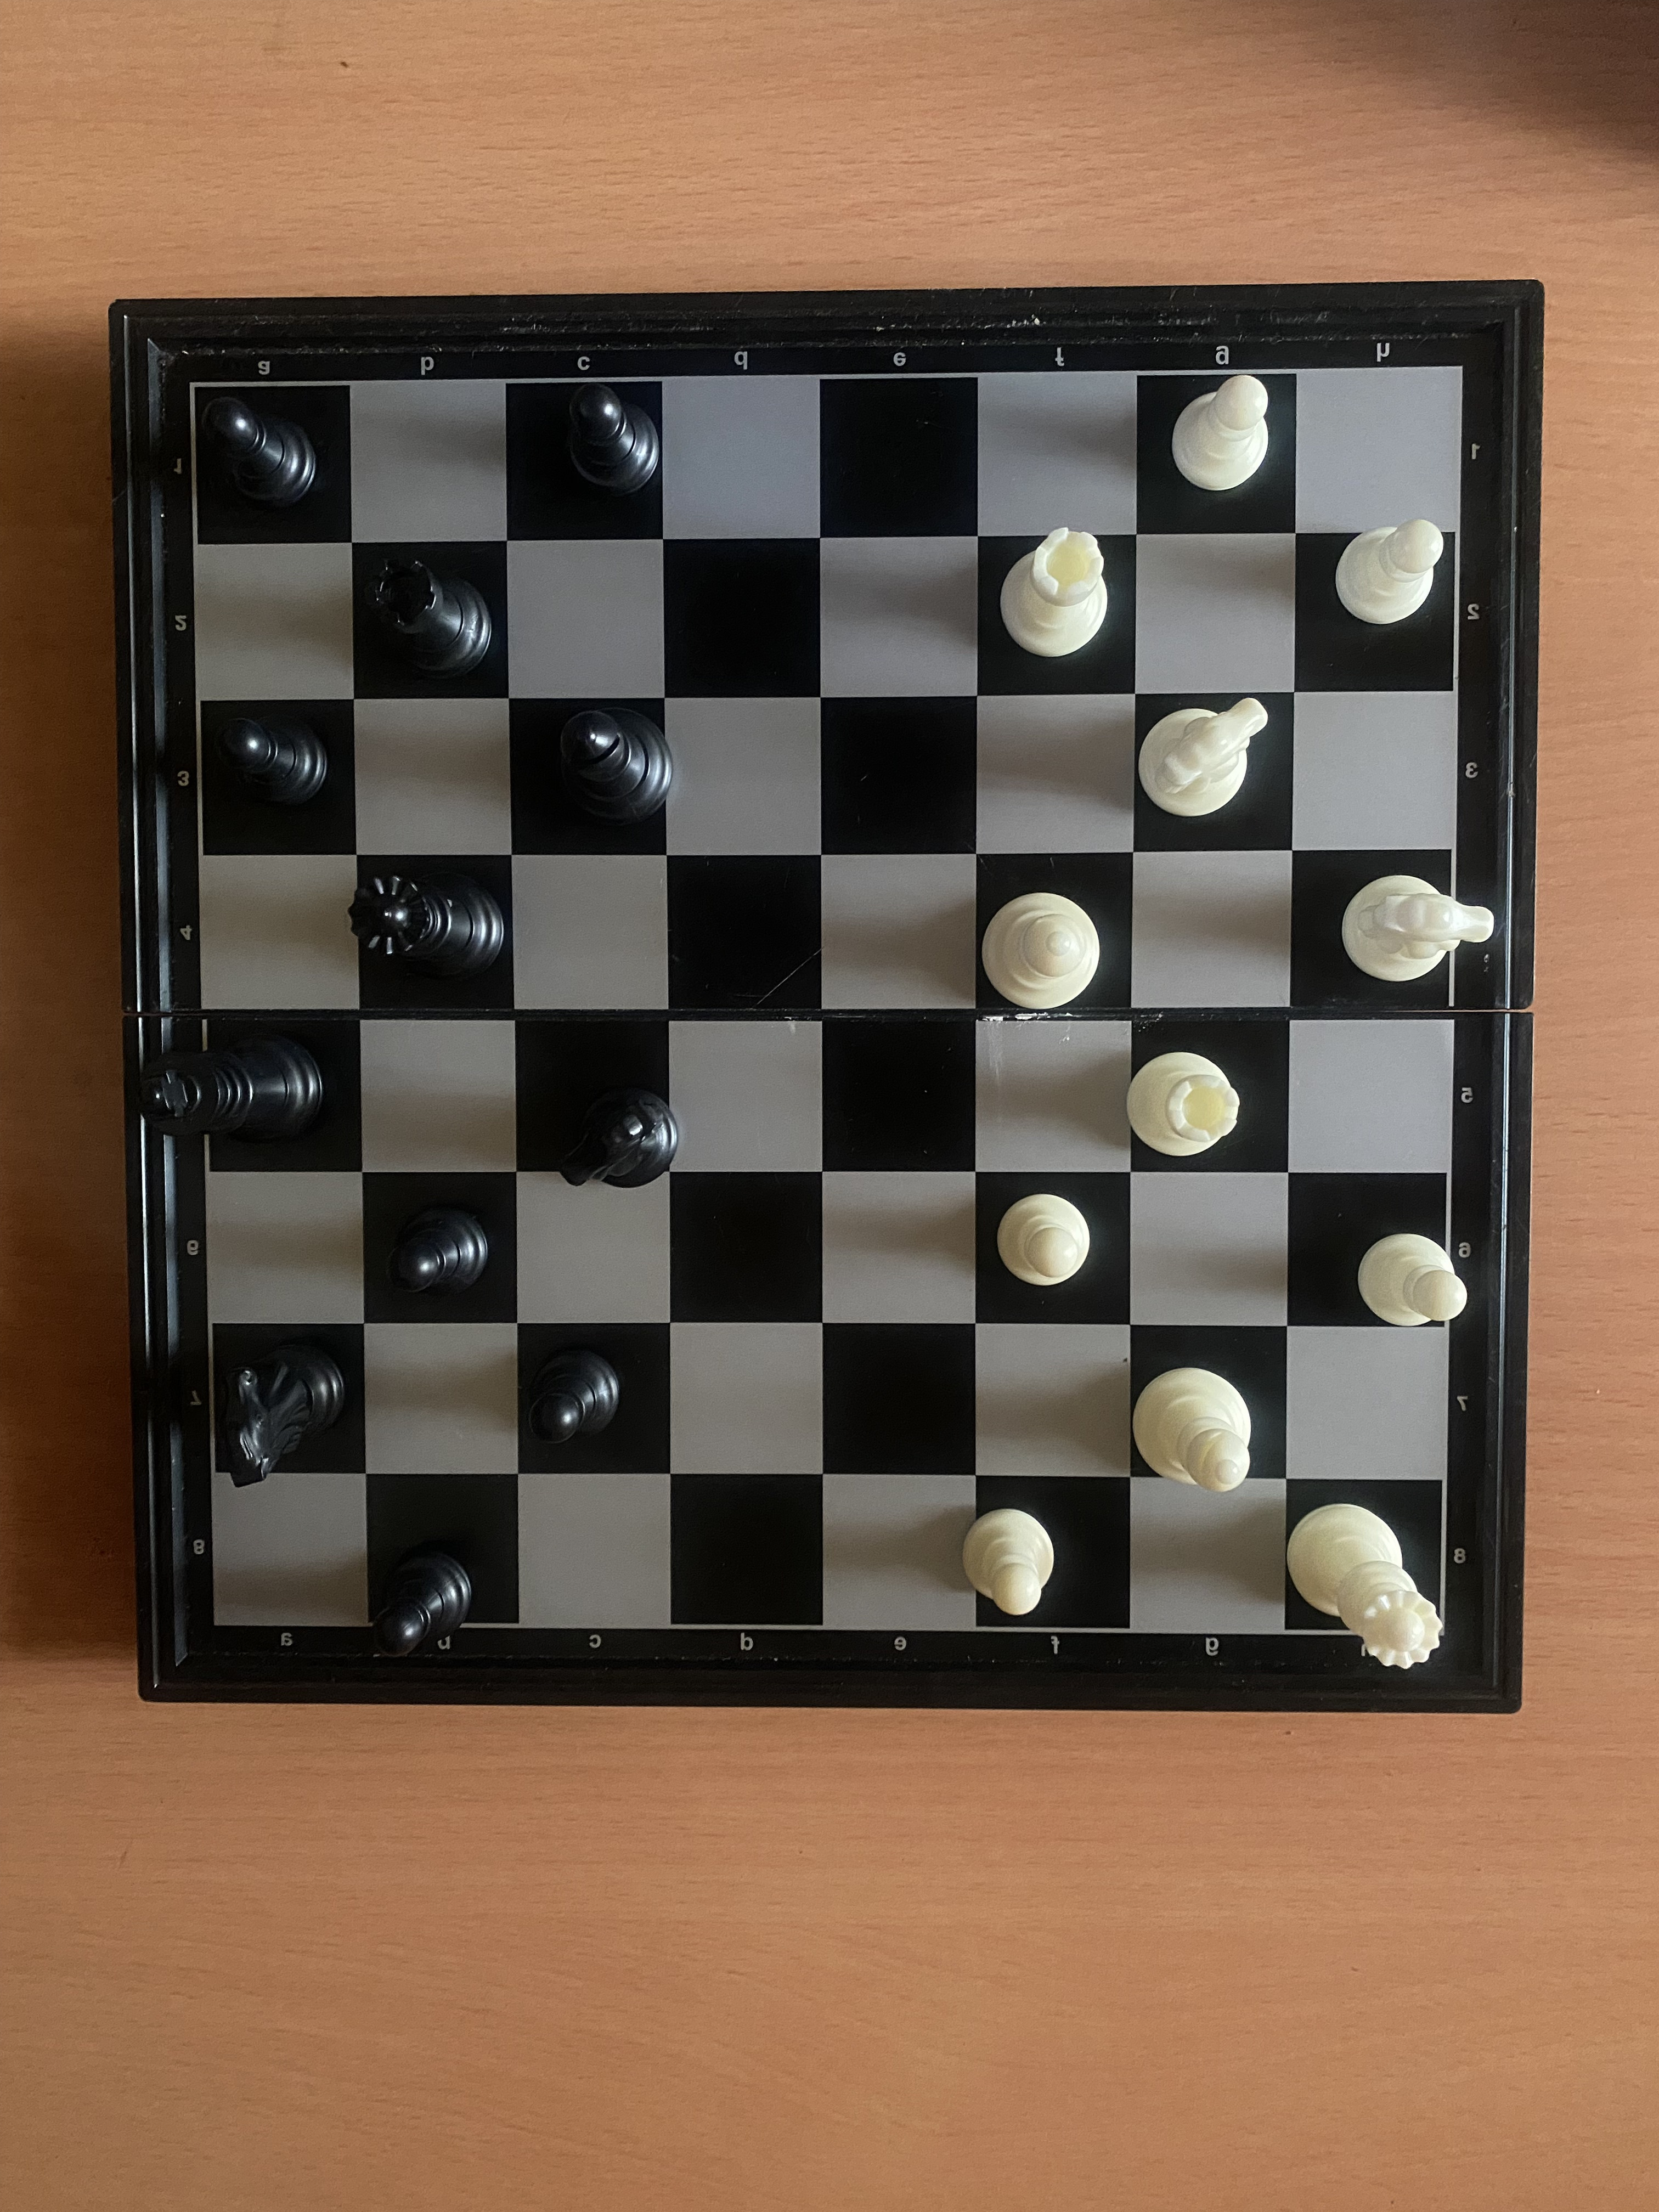
\includegraphics[width=\linewidth]{q4_vertical_flip.jpg}
        \caption{V-Flip}
    \end{subfigure}
    \hfill
    \begin{subfigure}[b]{0.19\textwidth}
        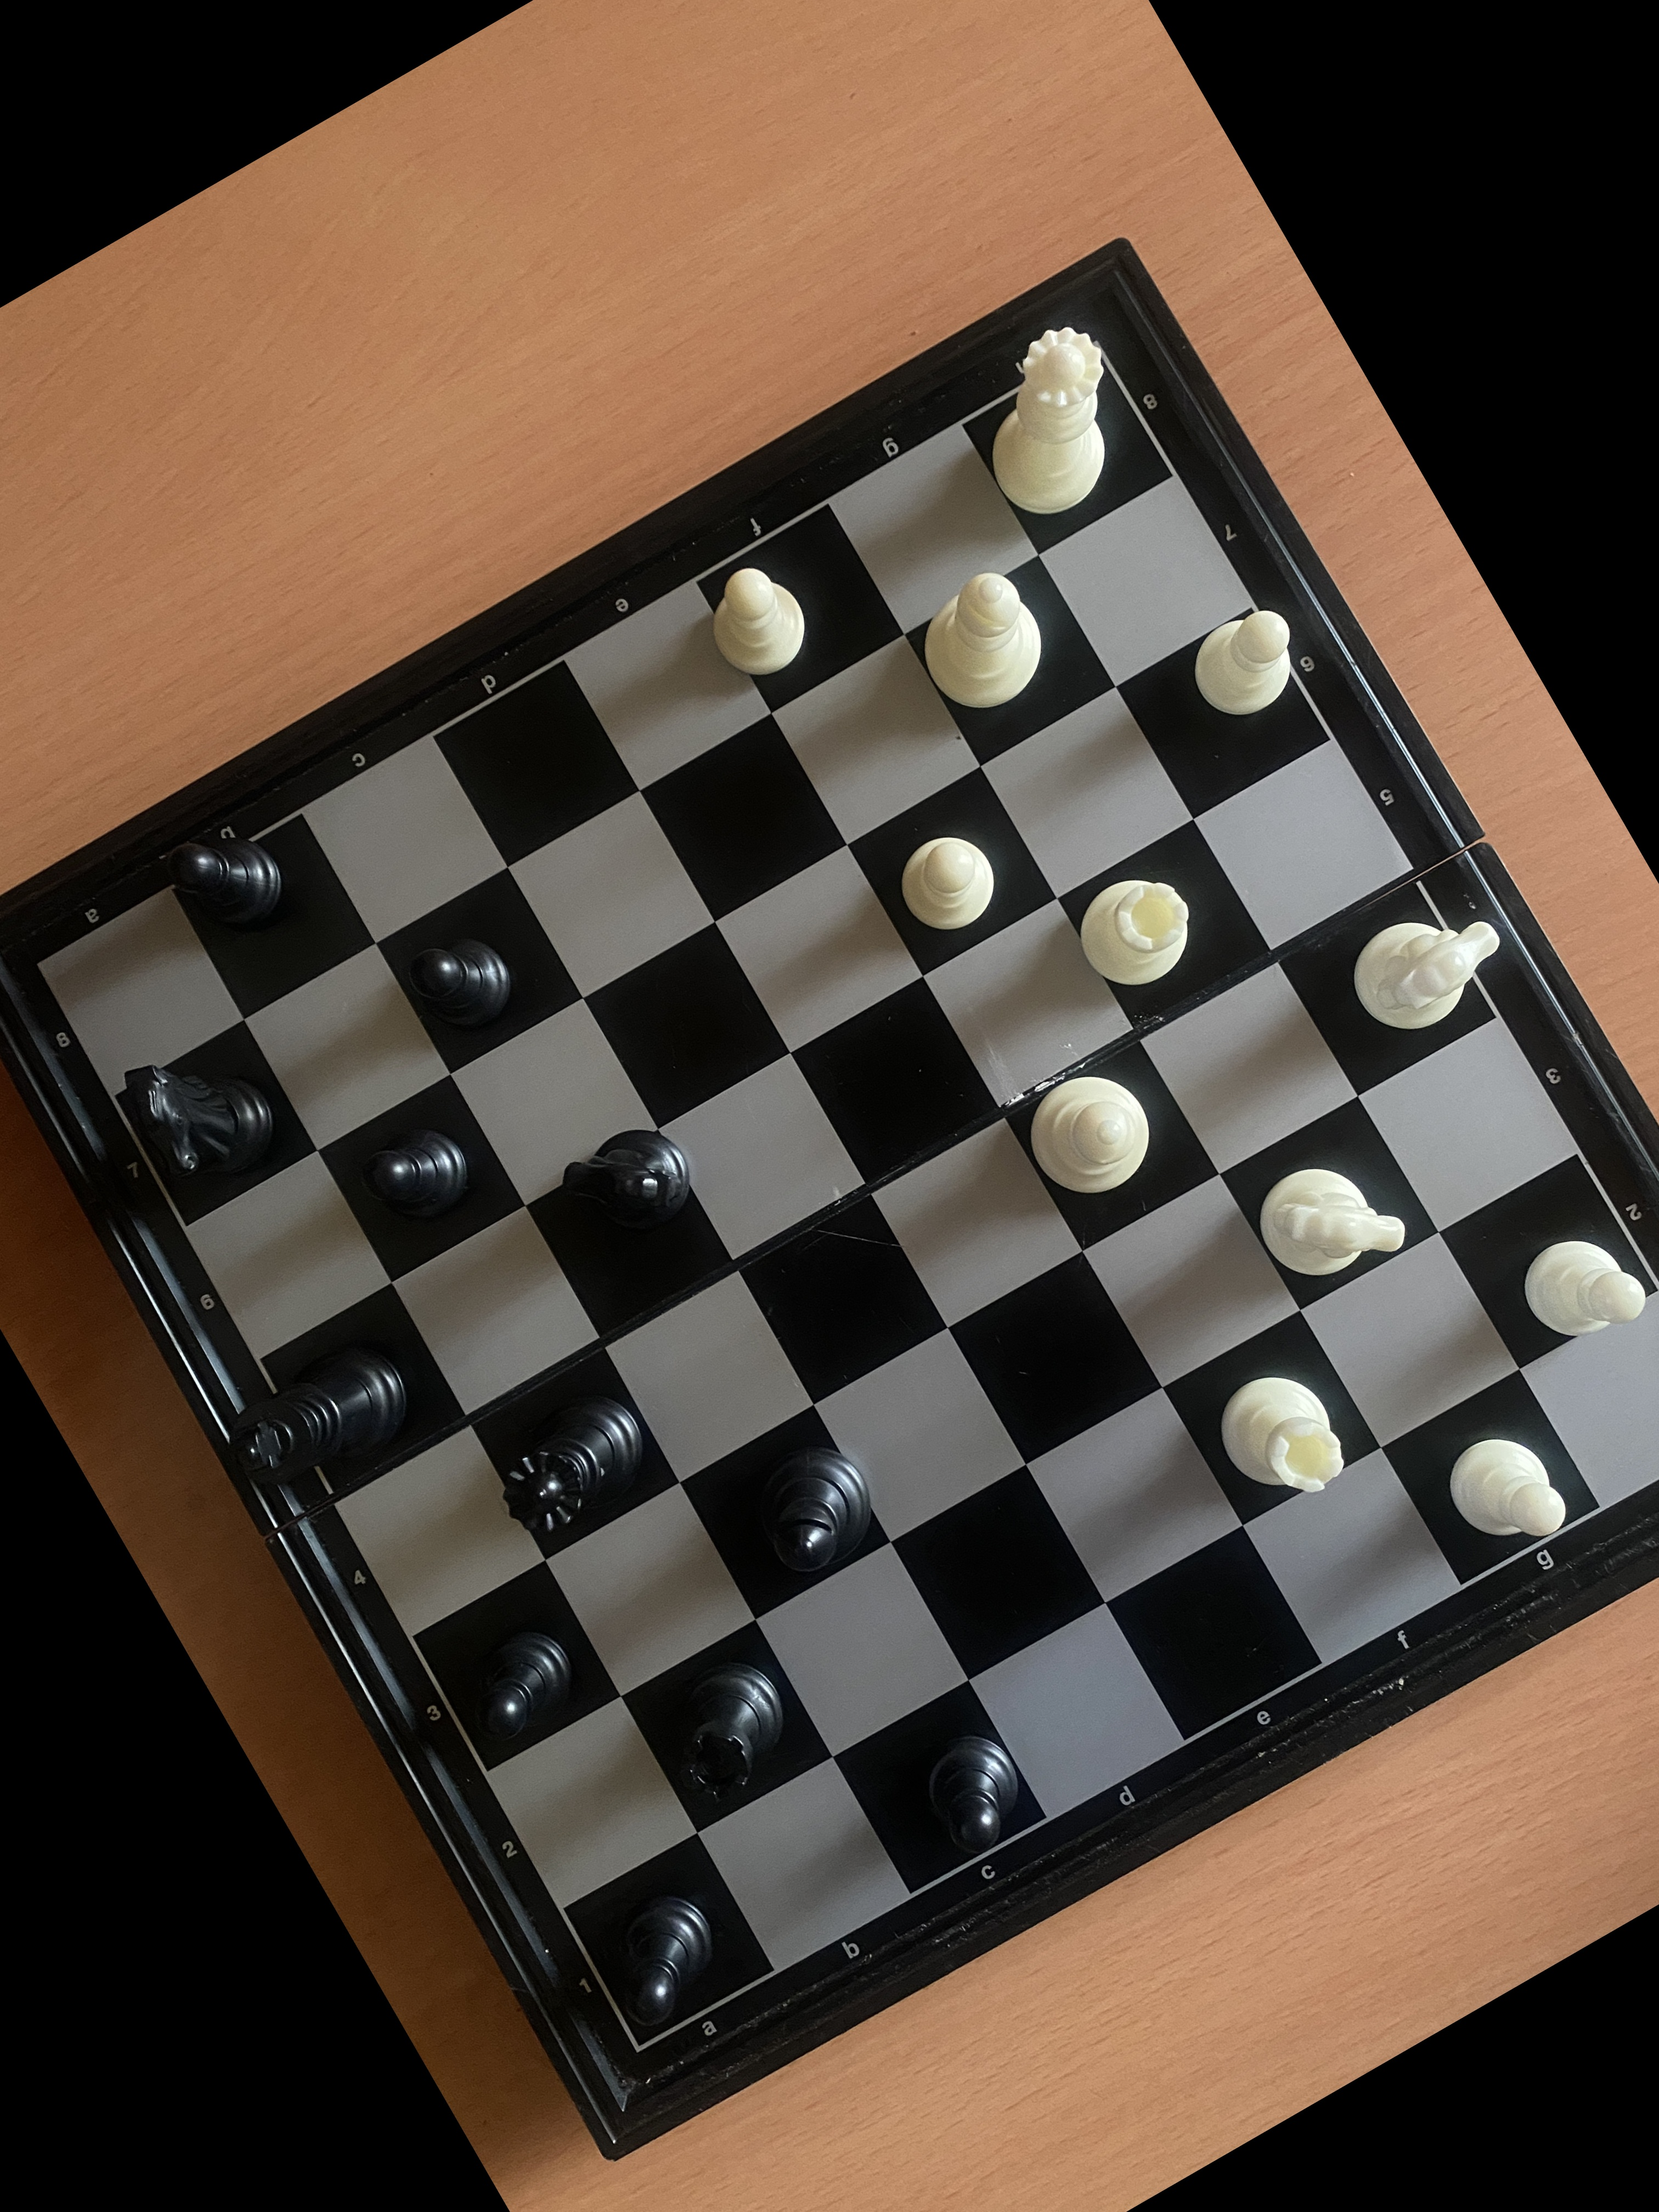
\includegraphics[width=\linewidth]{q4_rotation.jpg}
        \caption{Rotation ($30^\circ$)}
    \end{subfigure}
    \hfill
    \begin{subfigure}[b]{0.19\textwidth}
        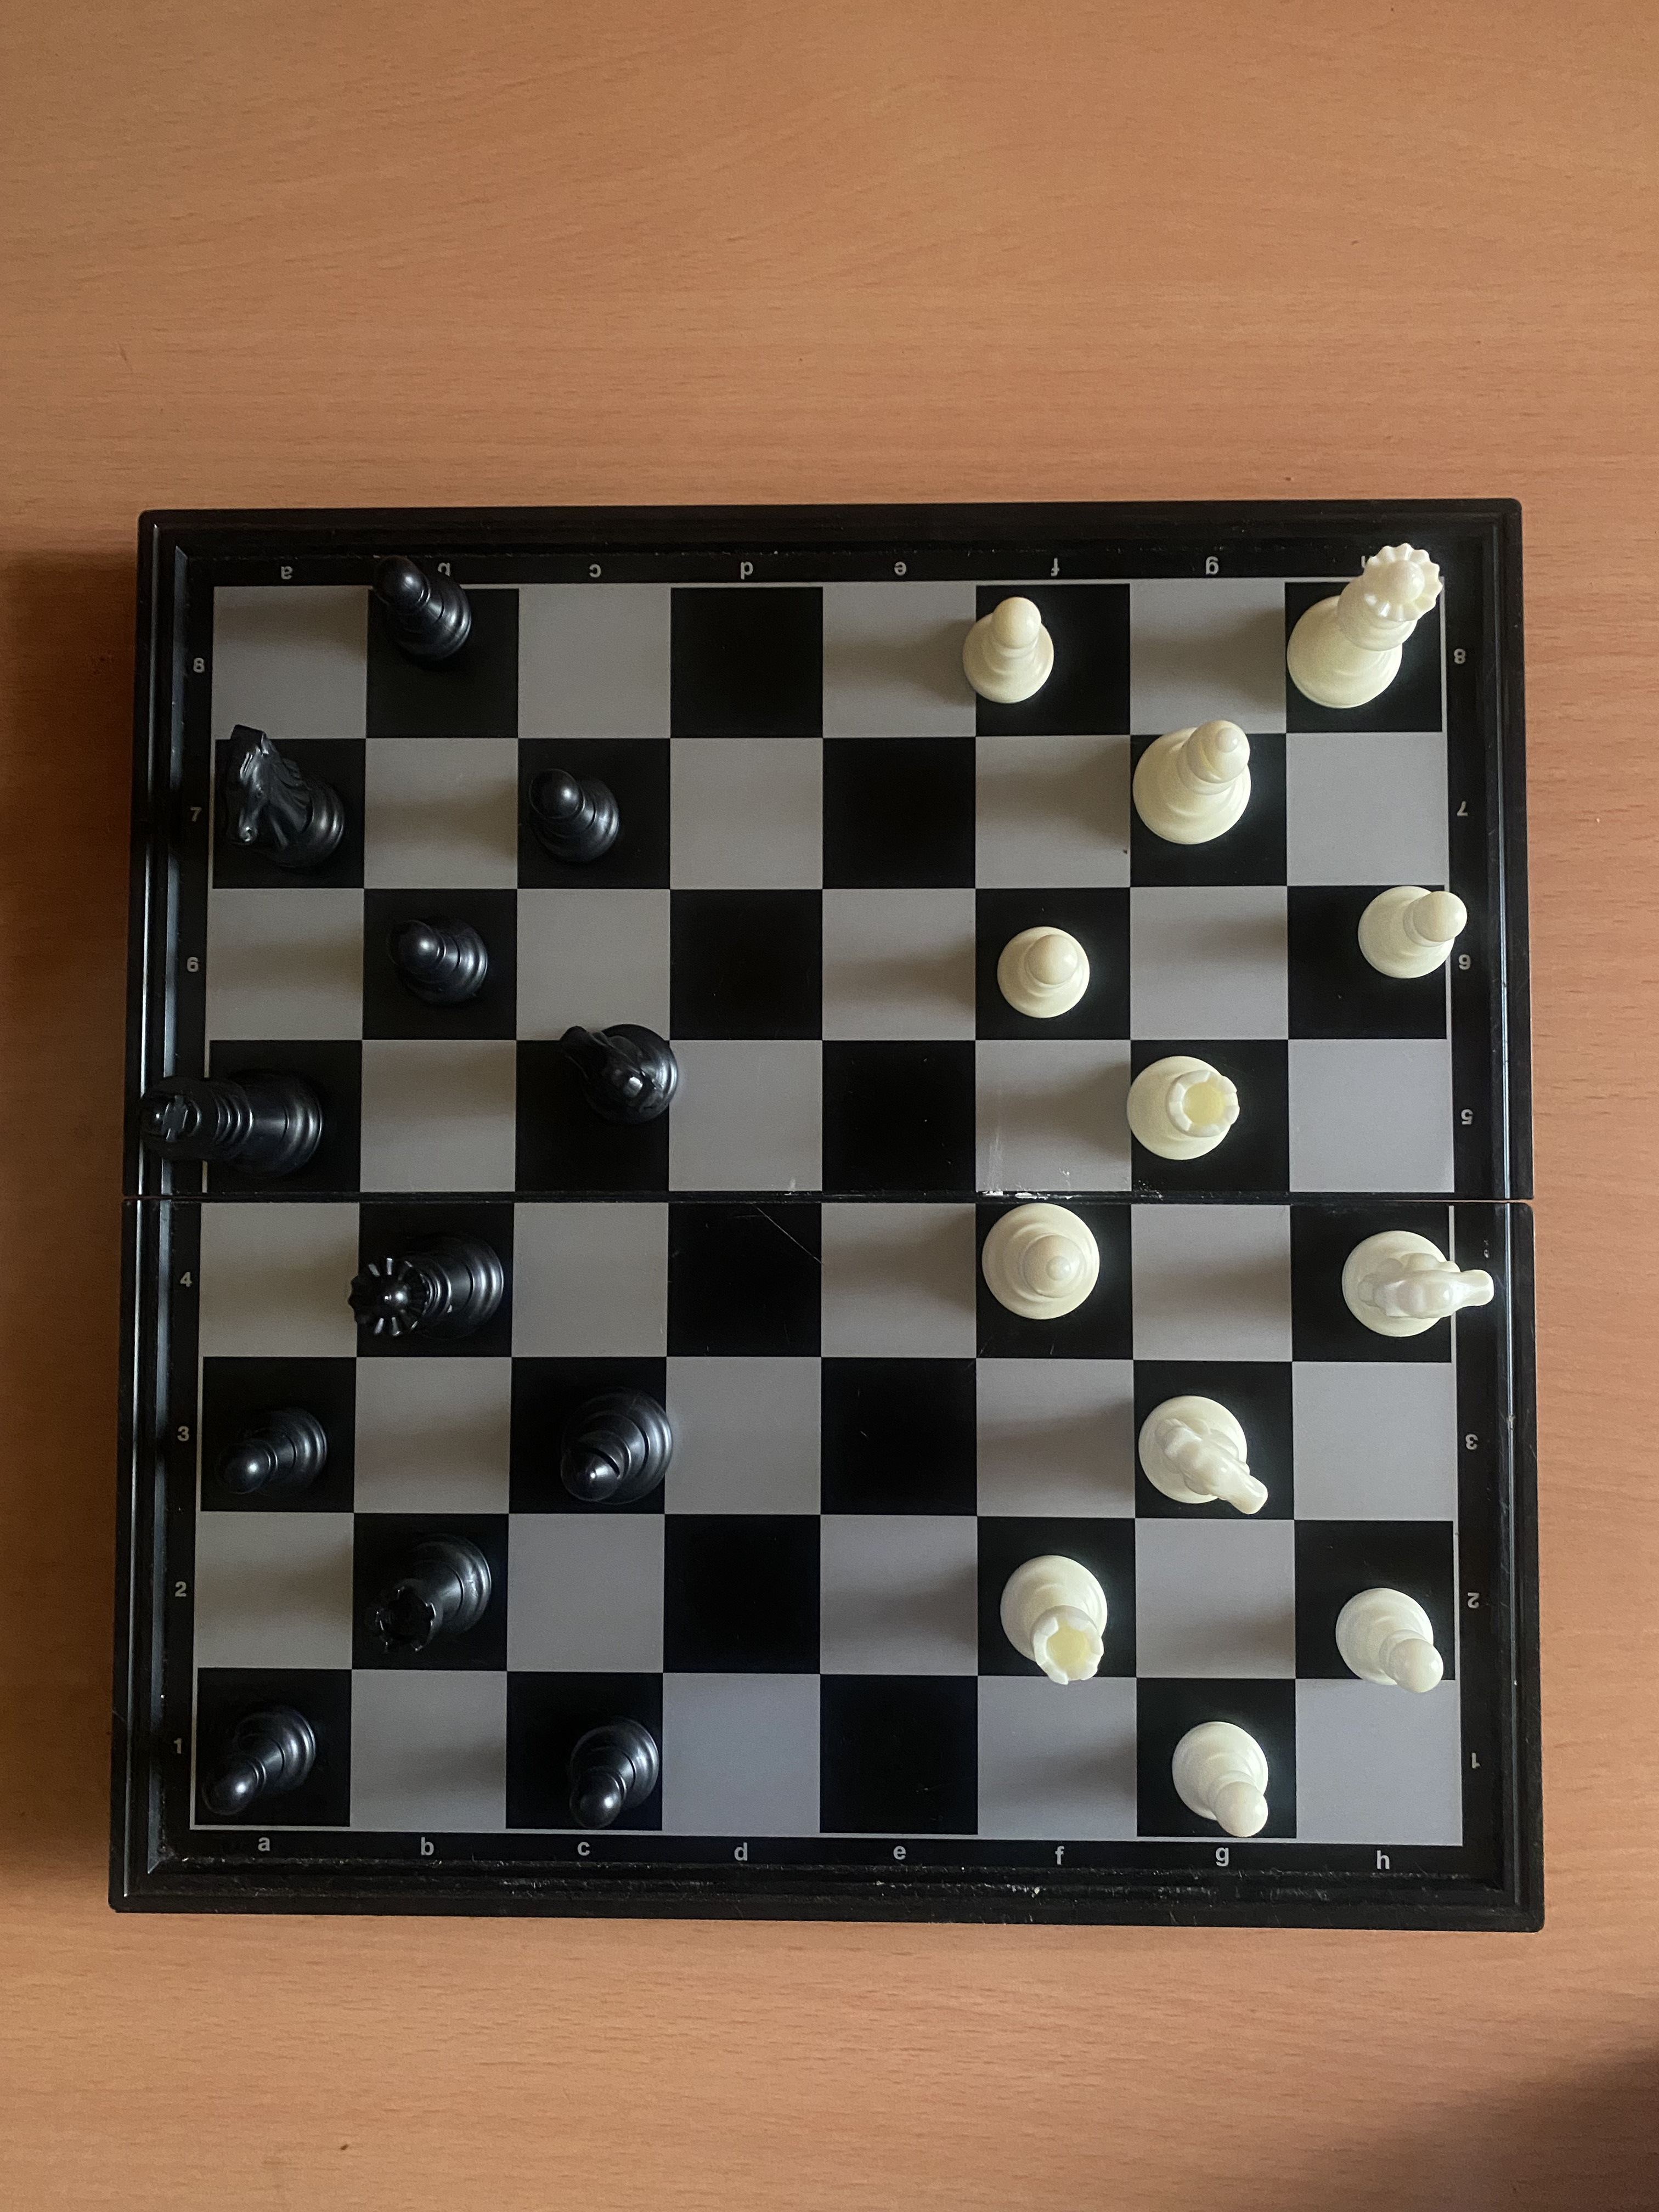
\includegraphics[width=\linewidth]{q4_shear_x.jpg}
        \caption{Shear X}
    \end{subfigure}
    \hfill
    \begin{subfigure}[b]{0.19\textwidth}
        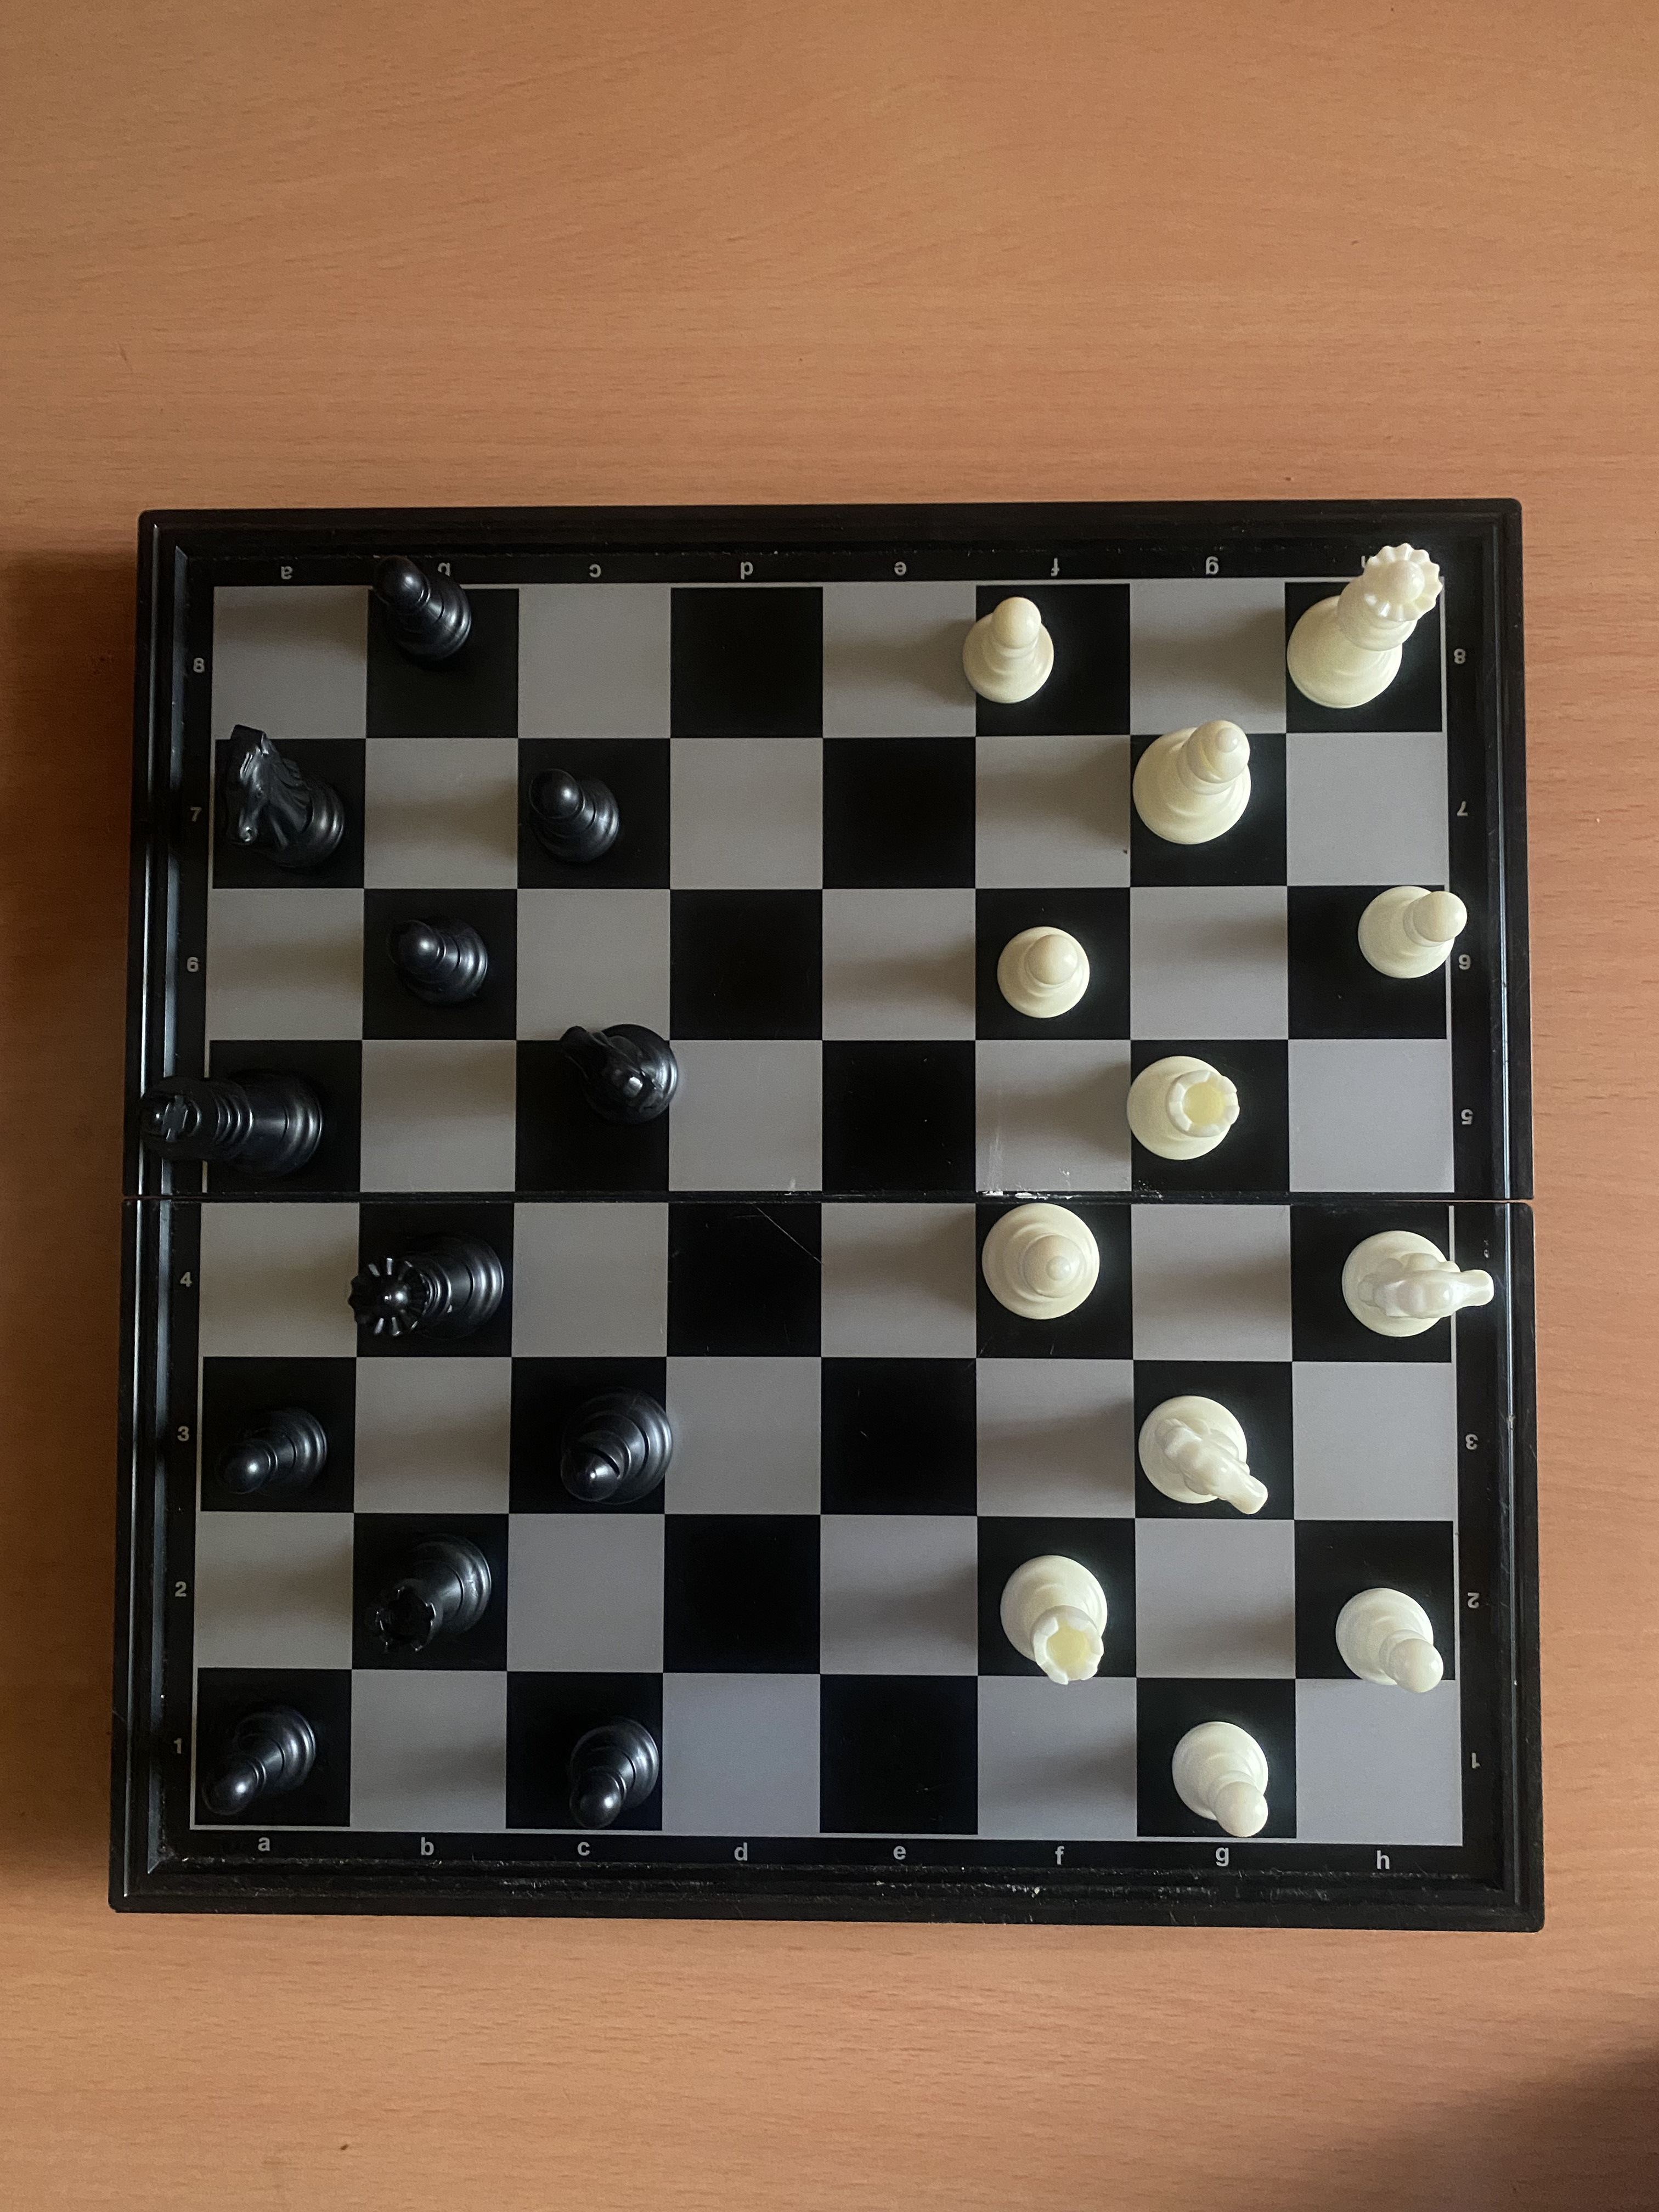
\includegraphics[width=\linewidth]{q4_shear_y.jpg}
        \caption{Shear Y}
    \end{subfigure}
    \caption{Data augmentation results applied to \texttt{2a.jpg}.}
    \label{fig:q4_results}
\end{figure}

\subsection{Validity for Face Recognition}
When applying augmentations to a dataset labeled ``Face'', we must consider if the transformation preserves the label's semantic validity~\cite{shorten2019survey}.
\begin{itemize}
    \item \textbf{Horizontal Flip is VALID:} A mirrored face is semantically identical to a real face (humans are roughly symmetric).
    \item \textbf{Vertical Flip is INVALID:} Upside-down faces are rare in natural environments. Validating on them might force the network to learn incorrect spatial relationships (e.g., eyes below mouth).
    \item \textbf{Rotation ($30^\circ$) is VALID:} Small rotations simulate head tilt, which is common.
    \item \textbf{Gaussian Blur is VALID:} Simulates out-of-focus images, improving robustness.
    \item \textbf{Shear is PARTIALLY VALID:} Slight perspective changes are good, but extreme shear distorts facial proportions unnaturally.
\end{itemize}
\subsection{Other Transforms}
Two other transforms not included in the starter code that are highly relevant for face recognition:
\begin{itemize}
    \item \textbf{Photometric Distortion (Brightness/Contrast):} Adjusting brightness and contrast is crucial~cite{sun2005geometric} because face recognition systems must be robust to varying lighting conditions, such as shadows, indoor/outdoor transitions, and overexposure.
    \item \textbf{Random Occlusion (Cutout):} Simulating partial occlusion~\cite{fong2019occlusions} (e.g., by masking out random rectangular regions) is essential for training models to recognize faces that may be partially covered by accessories like sunglasses, medical masks, or microphones.
\end{itemize}

\newpage
\bibliographystyle{ieeetr}
\nocite{*}
\bibliography{references}

\end{document}
